%----------------------------------------------------------------
%
%  File    :  thesis.tex
%
%  Authors :  Keith Andrews, IICM, TU Graz, Austria
%             Manuel Koschuch, FH Campus Wien, Austria
%			  Sebastian Ukleja, FH Campus Wien, Austria
% 
%  Created :  22 Feb 96
% 
%  Changed :  14 Oct 2020
%
%  For suggestions and remarks write to: sebastian.ukleja@fh-campuswien.ac.at
% 
%----------------------------------------------------------------

% --- Setup for the document ------------------------------------

%Class for a book like style:
\documentclass[11pt,a4paper,oneside]{scrbook}
%For a more paper like style use this class instead:
%\documentclass[11pt,a4paper,oneside]{thesis}

%input encoding for windows in utf-8 needed for Ä,Ö,Ü etc..:
\usepackage[utf8]{inputenc}
%input encoding for linux:
%\usepackage[latin1]{inputenc}
%input encoding for mac:
%\usepackage[applemac]{inputenc}

\usepackage[english]{babel}
% for german use this line instead:
%\usepackage[ngerman]{babel}

%needed for font encoding
\usepackage[T1]{fontenc}
\usepackage{float}

% want Arial? uncomment next two lines...
%\usepackage{uarial}
%\renewcommand{\familydefault}{\sfdefault}

%some formatting packages
\usepackage[bf,sf]{subfigure}
\renewcommand{\subfigtopskip}{0mm}
\renewcommand{\subfigcapmargin}{0mm}

%For better font resolution in pdf files
\usepackage{lmodern}

\usepackage{url}

%\usepackage{latexsym}

\usepackage{geometry} % define pagesize in more detail


\usepackage{colortbl} % define colored backgrounds for tables

\usepackage{courier} %for listings
\usepackage{listings} % nicer code formatting
\lstset{basicstyle=\ttfamily,breaklines=true}

\usepackage{graphicx}
  \pdfcompresslevel=9
  \pdfpageheight=297mm
  \pdfpagewidth=210mm
  \usepackage[         % hyperref should be last package loaded
    pdftex, 		   % needed for pdf compiling, DO NOT compile with LaTeX
    bookmarks,
    bookmarksnumbered,
    linktocpage,
    pagebackref,
    pdfview={Fit},
    pdfstartview={Fit},
    pdfpagemode=UseOutlines,                 % open bookmarks in Acrobat
  ]{hyperref}
\DeclareGraphicsExtensions{.pdf,.jpg,.png}
\usepackage{bookmark}

\usepackage[title]{appendix}

%paper format
\geometry{a4paper,left=30mm,right=25mm, top=30mm, bottom=30mm}

% --- Settings for header and footer ---------------------------------
\usepackage{scrlayer-scrpage}
\clearscrheadfoot
\pagestyle{scrheadings}
\automark{chapter}

%Left header shows chapter and chapter name, will not display on first chapter page use \ihead*{\leftmark} to show on every page
\ihead{\leftmark} 	
%\ohead*{\rightmark}	%optional right header
\ifoot*{Student}		%left footer shows student name
\ofoot*{\thepage}		%right footer shows pagination
%---------------------------------------------------------------------

%Start of your document beginning with title page
\begin{document}


% --- Main Title Page ------------------------------------------------
\begin{titlepage}
\frontmatter

\begin{picture}(50,50)
\put(-70,40){\hbox{
\includegraphics{images/logo.png}}}
\end{picture}

\vspace*{-5.8cm}

\begin{center}

\vspace{6.2cm}

\hspace*{-1.0cm} {\LARGE \textbf{Data Science and Visualisation Techniques applied on Bus Search Requests and its Correlating Booking Data\\}}
\vspace{0.2cm}
\hspace*{-1.0cm} Subtitle\\

\vspace{2.0cm}

\hspace*{-1.0cm} { \textbf{Bachelor Thesis\\}}

\vspace{0.65cm}

\hspace*{-1.0cm} Submitted in partial fulfillment of the requirements for the degree of \\

\vspace{0.65cm}

\hspace*{-1.0cm} \textbf{Bachelor of Science in Engineering\\}

\vspace{0.65cm}

\hspace*{-1.0cm} to the University of Applied Sciences FH Campus Wien \\
\vspace{0.2cm}
\hspace*{-1.0cm} Bachelor Degree Program: Computer Science and Digital Communications \\

\vspace{1.6cm}

\hspace*{-1.0cm} \textbf{Author:} \\
\vspace{0.2cm}
\hspace*{-1.0cm} first name surname \\

\vspace{0.7cm}

\hspace*{-1.0cm} \textbf{Student identification number:}\\
\vspace{0.2cm}
\hspace*{-1.0cm} Number \\

\vspace{0.7cm}

\hspace*{-1.0cm} \textbf{Supervisor:} \\
\vspace{0.2cm}
\hspace*{-1.0cm} Title first name surname \\

\vspace{0.7cm}

% Reviewer if needed
%\hspace*{-1.0cm} \textbf{Reviewer: (optional)} \\
%\vspace{0.2cm}
%\hspace*{-1.0cm} Title first name surname \\


\vspace{1.0cm}

\hspace*{-1.0cm} \textbf{Date:} \\
\vspace{0.2cm}
\hspace*{-1.0cm} dd.mm.yyyy \\

\end{center}
\end{titlepage}

\newpage

\vspace*{16cm}
\setcounter{page}{1}

% --- Declaration of authorship ------------------------------------------
\hspace*{-0.7cm} \underline{Declaration of authorship:}\\\\
I declare that this Bachelor Thesis has been written by myself. I have not used any other than the listed sources, nor have I received any unauthorized help.\\\\
I hereby certify that I have not submitted this Bachelor Thesis in any form (to a reviewer for assessment) either in Austria or abroad.\\\\
Furthermore, I assure that the (printed and electronic) copies I have submitted are identical.
\\\\\\
Date: \hspace{6cm} Signature:\\

% --- English Abstract ----------------------------------------------------
\cleardoublepage
\chapter*{Abstract}
(E.g. ``This thesis investigates...'')

% --- German Abstract ----------------------------------------------------
\cleardoublepage
\chapter*{Kurzfassung}
(Z.B. ``Diese Arbeit untersucht...'')


% --- Abbrevations ----------------------------------------------------
\chapter*{List of Abbreviations}
\vspace{0.65cm}

\begin{table*}[htbp]
		\begin{tabular}{ll}
			ARP & Address Resolution Protocol \\
			GPRS & General Packet Radio Service \\
			GSM  &  Global System for Mobile communication \\
			WLAN & Wireless Local Area Network \\
		\end{tabular}
\end{table*}

% --- Key terms ----------------------------------------------------
\newpage
\chapter*{Key Terms}
\vspace{0.65cm}

\begin{itemize}
	\setlength{\itemsep}{0pt}
	\item[] GSM
	\item[] Mobilfunk
	\item[] Zugriffsverfahren
\end{itemize}

% --- Table of contents autogenerated ------------------------------------
\newpage
\tableofcontents
\thispagestyle{empty}

% --- Begin of Thesis ----------------------------------------------------
\mainmatter
%----------------------------------------------------------------
%
%  File    :  introduction.tex
%
%  Authors : Thomas Lerchbaumer
% 
%  Created :  19 March 2022
% 
%  Changed :  19 March
% 
%----------------------------------------------------------------

\chapter{Introduction}
\label{chap:introduction}
The rise of Machine Learning (ML), and especially Neural Networks (NN), has created so far unheard-of capabilities for predictive analysis when looking at individual traffic in the modern transportation landscape. As digitalization emerged rapidly over the past years the possibilities for data-driven decision making further evolved as well. In general data-driven decision making is a process which involves collecting data to measure goals or Key Performance Indicators (KPIs). Furthermore data gathered through business processes can also be consulted in order to support business owners during their decision making process.
\newline
\newline
Predictive analysis involves statistical techniques and ML algorithms to analyse current as well as historical information in order to predict future events. The applications of predictive analysis span various sectors and industries. In finance it can be utilised to predict stock market trends \cite{stock_market}. When looking at healthcare it can assist in predicting diseases and to support doctors in their diagnosis \cite{health_care}. In retail it can help to understand customer behaviours \cite{retail}. How well certain algorithms can perform is influenced by the quality of available data \cite{data_qual}. In recent years ML techniques, especially NN, demonstrated promising results when it comes to time series forecasting. Certain NN models have the ability to detect non-linear relationship within a given dataset. Recurrent Neural Networks (RNN)including Long Short-Term Memory (LSTM) are commonly used approaches in this area as they have the ability to capture long term dependencies \cite{intro_ml_1}.
\newline
\newline
Furthermore each company has to measure their Key Performance Indicators (KPIs). Those KPIs reflect a company's short and long-term goals. Keeping track of them help companies to see how they perform against their goals and to carry out adjustments whenever needed.\cite{kpi_imrpove_businiess} To stay competitive, one crucial aspect is how this gathered data can be accessed and analysed. One very simple approach is to manually calculate defined KPIs when needed. As this process is rather time consuming a different approach is to provide Business Indicators Management (BIM) \cite{kpi_imrpove_decision_making}. Such systems are usually software based and lay the fundamentals for data driven decision making, as they come along with several advantages. They reduce the time required to analyse indicators which are necessary for decisions. Additionally various filters can be applied to data in real time which improves the agility when analysing data. As those analytical dashboards often use various visualisation methods ranging from simple plots to interactive maps unseen trends and insights become visible.\cite{kpi_imrpove_decision_making}
\newline
\newline 
One crucial element for every business is to stay ahead of their competitors. Depending on the industry a company operates in, those strategies may vary but the utilisation of data is one key element to successfully put strategies into practice.
In context of individual transportation one key factor is to continuously improve the offered service.****CITEHERE**** Therefore data gathered from a digital booking platform like busfinder can reveal valuable information like customer preferences, preferred travel times, common departure and destination places as well as seasonal booking patterns.
\newline
\newline
As busfinder acts as interface between bus operators and their clients considerations about both parties have to be made whenever improvements are set in place. One improvement that favours both parties is Yield Management. For customers the utilisation of YM results in a higher price flexibility and transparency. Whereas operators can use it to maximise their revenue and to improve their efficiency when it comes to resource utilisation.\cite{yield_m} As the offered service from busfinder includes the complete route planning as well as the whole booking and payment process a vast amount of data is gathered in order to process customer requests. Furthermore plain search requests that do no result in a booking are also stored and usable for analytical purposes.
\newline
\newline
Busfinder strives to optimise its offered service by utilising the available data described during chapter \ref{chap:available_dataset}. The aim of this paper is to figure out what Neural Networks (NNs) are suitable to predict future bus bookings in order to improve the current YM and which attributes of bus search requests can be utilised to contribute to an analytical dashboard. To carry out which NNs and models are the most promising for time series forecasting a literature review is conducted. Furthermore the evaluated models are implemented to measure their performance. Both the implementation as well as the literature review are discussed during chapter \ref{chap:predict}. Additionally the search requests are analysed for metrics that support operators that follow a data driven decision approach. The theory on how to conduct such an analysis was covered in the author's previous thesis. The gathered insights and their implementation are explained during chapter \ref{chap:analytical_dashboard}.


 
%----------------------------------------------------------------
%
%  File    :  lit_research.tex
%
%  Authors : Thomas Lerchbaumer
% 
%  Created :  19 March 2022
% 
%  Changed :  19 March
% 
%----------------------------------------------------------------

\chapter{Info}
\label{chap:info}

\subsection{Research Question}
What Neural Networks are suitable to predict future bus bookings and which attributes of bus search requests can be utilized to create an analytical dashboard.


Research Question BA1: How to create a theoretical framework that covers basic DS
aspects and visualization techniques in order to develop an analytical web-based dashboard



\subsection{General}
Basic Idea/Content: \newline

\begin{itemize}
  \item Explain available dataset, data structure, how data is gathered 
  \item Explain what techniques are used to clean the base dataset
  \item Interdisciplinary - explain why certain KPIs or models are choosen and are applied onto the dataset 
  \item Prediction Model - explain the technologies, methods etc. used to create a ML based prediction model (To improve Yield Management). Maybe two models, Supervised Learning and unsupervised learning 
  \item Data Clustering and other KPIs + applied statistical models (e.g. Clustering, LR), Heatmaps etc. 
  \item Visualisation techniques used to display results of the applied statistical models 
  \item Maybe? Short chapter about technical setup of the Dashboard   
\end{itemize}
In general i would appreciate some general feedback what else could/should be descriped within this thesis. I think the Prediction Model will be the main aspect of this thesis (How it is created + which techniques are used, how is the performance when comparing prediction to actual booking data etc.) 




\subsection{Lit Research}
\cite{review_ml_styles} - provides also a lot of useful references to other papers that can be used 
\newline
\cite{prediction_stock_market} - ML 
\newline
\cite{hands_on_ML}, \cite{intro_ml}, \cite{tf_ctr},  \cite{bd_tf_price_forecasting} - Tensorflow, ML etc. 
\newline
\cite{kpi_imrpove_businiess}, \cite{kpi_imrpove_decision_making} - interdisciplinary to provide context which KPI's etc are chosen etc. 


%----------------------------------------------------------------
%
%  File    :  available_dataset.tex
%
%  Authors : Thomas Lerchbaumer
% 
%  Created :  19 March 2022
% 
%  Changed :  19 March 2022
% 
%----------------------------------------------------------------

\chapter{Available Dataset}
\label{chap:introduction}
general Infos

\section{Data Origin}
Where does the data come from (how it is gathered etc, important to explain the necessary data cleansing), how is it stored, for which purpose is it used. 
\section{Data Structure}
Avaiable attributes within the dataset, which attributes can be used for statistical purposes etc.
\section{Data Cleansing}
Which parameters are applied to the Dataset in order to clean it
\section{Possible Analytical Strageties that can be applied }

Explain what can be applied to the dataset, what procsses could be improved by analysing the data. 

Improve Yield Managment  (Prediction Model, ML) 


%%----------------------------------------------------------------
%
%  File    :  kpi.tex
%
%  Authors : Thomas Lerchbaumer
% 
%  Created :  19 March 2022
% 
%  Changed :  19 March
% 
%----------------------------------------------------------------

\chapter{Key Performance Indicators and Yield Management}
\label{chap:kpi}



\subsection{Yield Management}
What Neural Networks are suitable to predict future bus bookings and which Attributes of bus search requests can be utilized to created a analytical dashboard


Research Question BA1: How to create a theoretical framework that covers basic DS
aspects and visualization techniques in order to develop an analytical web-based dashboard



\subsection{General}
Basic Idea/Content: \newline

\begin{itemize}
  \item Explain available dataset, data structure, how data is gathered 
  \item Explain what techniques are used to clean the base dataset
  \item Interdisciplinary - explain why certain KPIs or models are choosen and are applied onto the dataset 
  \item Prediction Model - explain the technologies, methods etc. used to create a ML based prediction model (To improve Yield Management). Maybe two models, Supervised Learning and unsupervised learning 
  \item Data Clustering and other KPIs + applied statistical models (e.g. Clustering, LR), Heatmaps etc. 
  \item Visualisation techniques used to display results of the applied statistical models 
  \item Maybe? Short chapter about technical setup of the Dashboard   
\end{itemize}
In general i would appreciate some general feedback what else could/should be descriped within this thesis. I think the Prediction Model will be the main aspect of this thesis (How it is created + which techniques are used, how is the performance when comparing prediction to actual booking data etc.) 




\subsection{Lit Research}
\cite{review_ml_styles} - provides also a lot of useful references to other papers that can be used 
\newline
\cite{prediction_stock_market} - ML 
\newline
\cite{hands_on_ML}, \cite{intro_ml}, \cite{tf_ctr},  \cite{bd_tf_price_forecasting} - Tensorflow, ML etc. 
\newline
\cite{kpi_imrpove_businiess}, \cite{kpi_imrpove_decision_making} - interdisciplinary to provide context which KPI's etc are chosen etc. 


%----------------------------------------------------------------
%
%  File    :  prediction_model.tex
%
%  Authors : Thomas Lerchbaumer
% 
%  Created :  19 March 2022
% 
%  Changed :  19 March
% 
%----------------------------------------------------------------

\chapter{Predicting Future Bookings}
\label{chap:predict}
As this paper aims at evaluation various NNs regarding their usage for time series forecasting this chapter explains which NNs are suitable and how they can be integrated. The knowledge of potential future bookings provide useful insights when it comes to YM. YM in general describes controlling price and capacity control in a simultaneous ways \cite{yield_m}. Therefore those predictions can be used to support bus operators in their pricing strategy. This chapter focuses on creating two prediction models utilising different techniques based on the data that is available. 
Both models are implemented using Python and the following libraries:
\begin{itemize}
\item  \verb|matplotlib|\footnote{https://matplotlib.org/} - used for plotting
\item \verb|pandas|\footnote{https://pandas.pydata.org/} - used for data manipulation 
\item \verb|tensorflow|\footnote{https://www.tensorflow.org/} - provides ML models
\item \verb|keras|\footnote{https://keras.io/} - Neural Network library
\end{itemize}

As there are various models available a literature review is conducted to figure out which models fit the purpose of time series forecasting. It turns out that the most promising NNs that can be utilised for time series prediction are either Convolutional Neural Networks (CNN) or Recurrent Neural Networks (RNN) especially Long Short-Term Memory (LSTM)\cite{nn_1}\cite{nn_2}\cite{lstm_1}\cite{lstm_2} \citep{rnn_time_series_predict}.

\section{Backpropagation}
\label{sec:bp}

As both of the models LSTM and CNN use Backpropagation (BP) for its training the basic concepts of the algorithm are explained in this section. To understand the logic of BP a few terms need a detailed explanation: 
\subsubsection{Gradient}
The gradient also called gradient descent is an algorithm that is used to optimise the loss function within BP. That means that the gradient descent indicates by how much the weights and biases need to be adjusted in order to reduce the actual error value which is the result of the applied loss function. \cite{bp_basic}
\subsubsection{Bias}
The bias is an additional parameter used in each neuron of a NN. It is used to directly influence the activation function to offset the results either to the negative or positive direction. When looking at the sigmoid function without any bias in place where \verb|x| correlates to the input value and \verb|w| indicates the used weight: 
\begin{equation}
 \sigma(x) = \frac{1} {1 + e^{-{(w*x)}}}
\label{eq:eq_4}
\end{equation}
When looking at figure \ref{fig:sig_wo_bias} the weights only influence the steepness of the function but will not shift it along the x axes.
\begin{figure}[H]
	\centering
		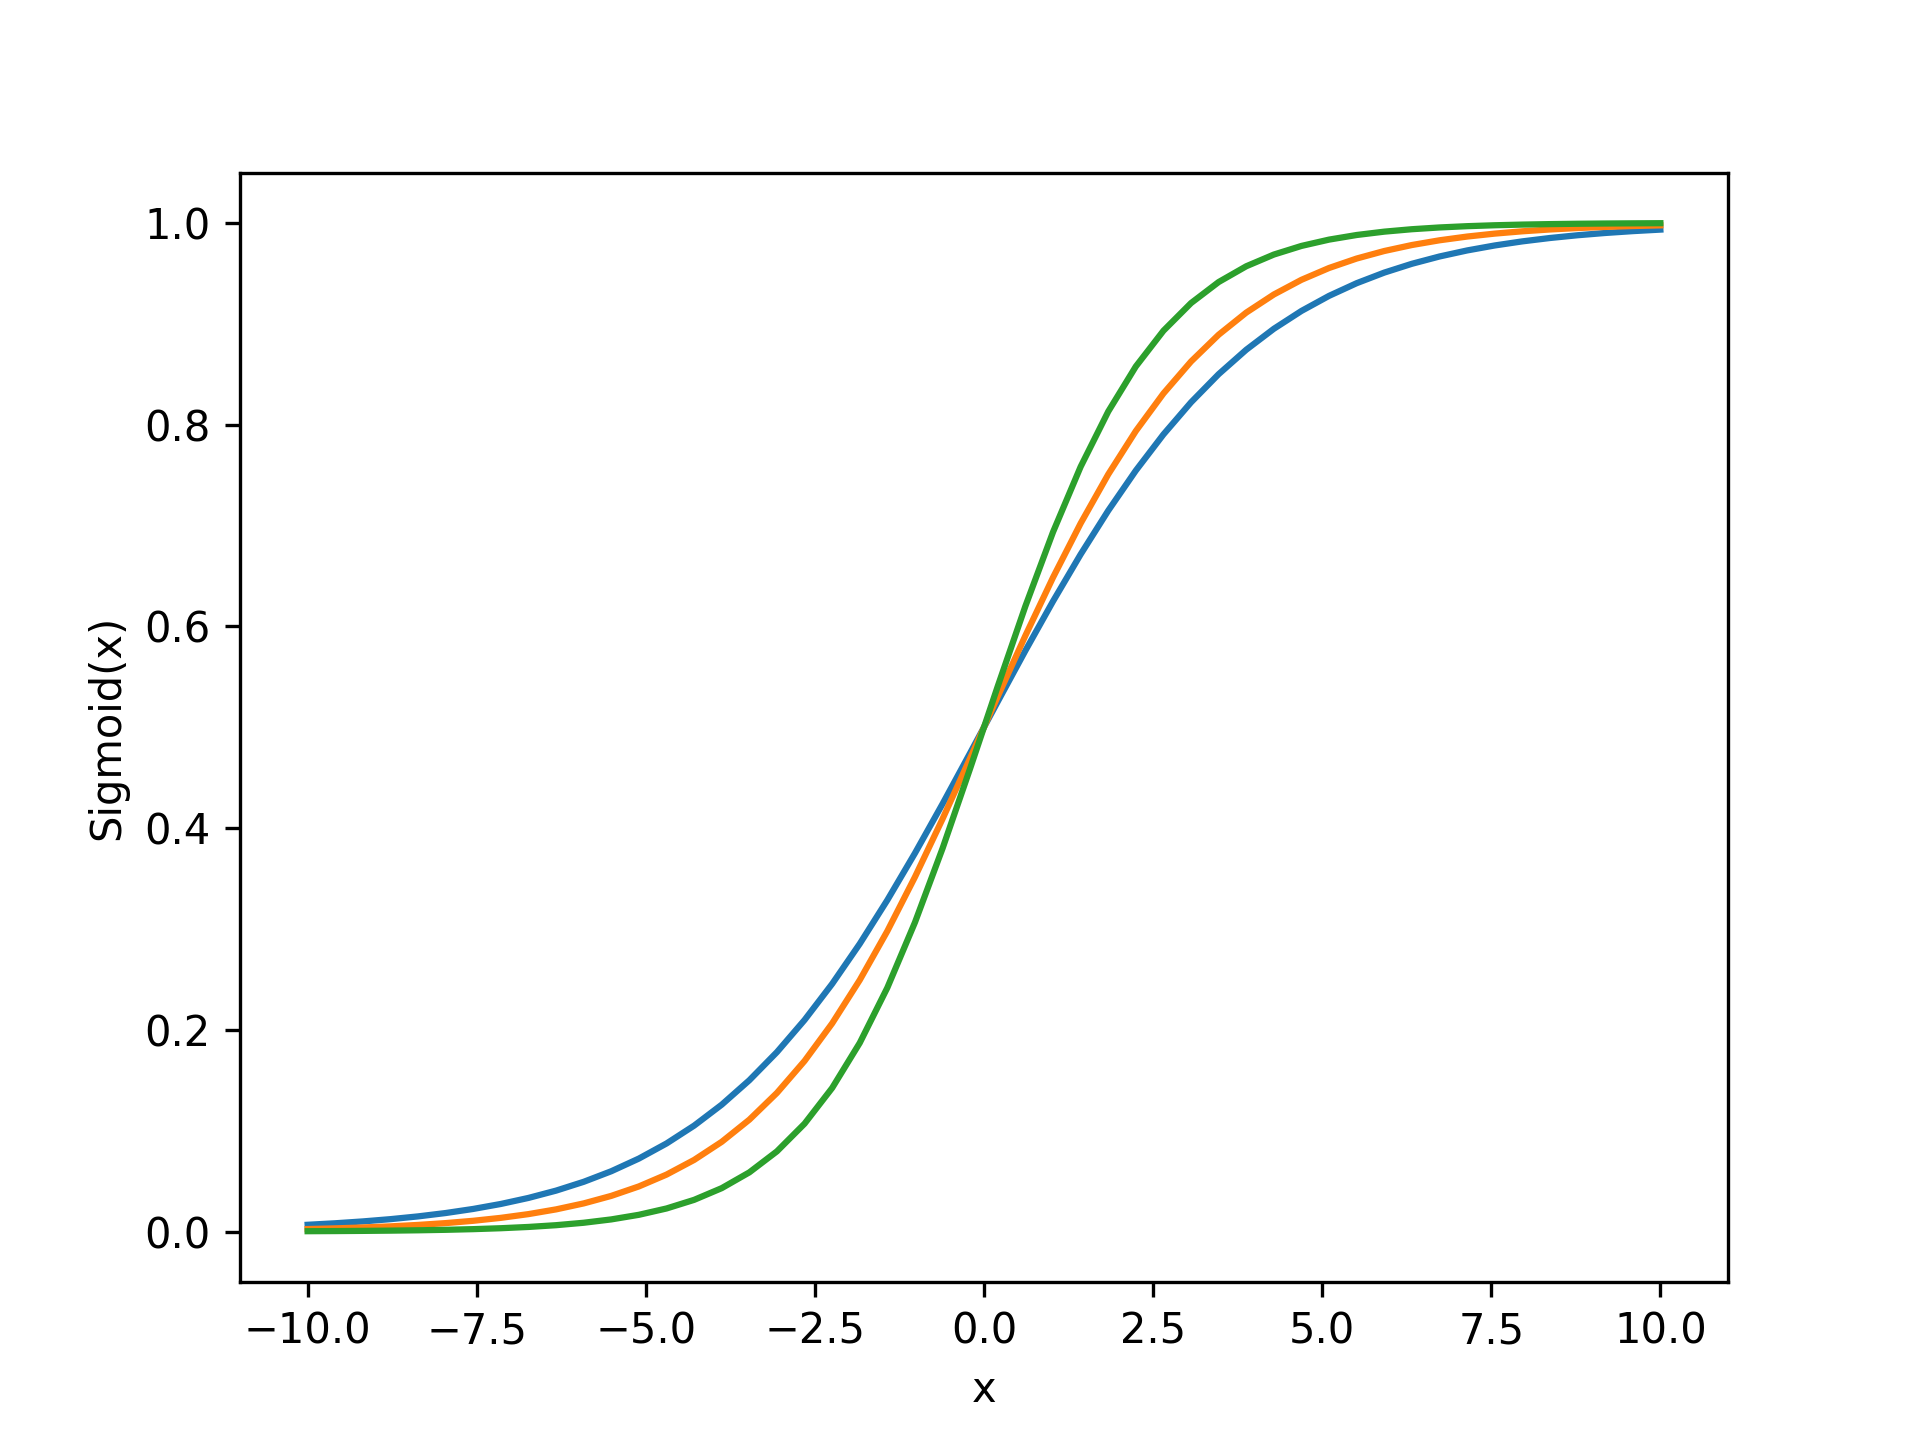
\includegraphics[width=8cm]{images/sigmoid_w_weights}
	\caption{Sigmoid function with different weights and no bias - [source:\cite{lstm_module}]}
	\label{fig:sig_wo_bias}
\end{figure}
 To shift the function along the x axes the sigmoid function is adapted with the bias \verb|b| value: 
\begin{equation}
 \sigma(x) = \frac{1} {1 + e^{-{(w*x+b)}}}
\label{eq:eq_4}
\end{equation}
By adding the bias value as constant to the sigmoid function can be shifted along the x axes as shown in figure \ref{fig:sig_w_bias}.
\begin{figure}[H]
	\centering
		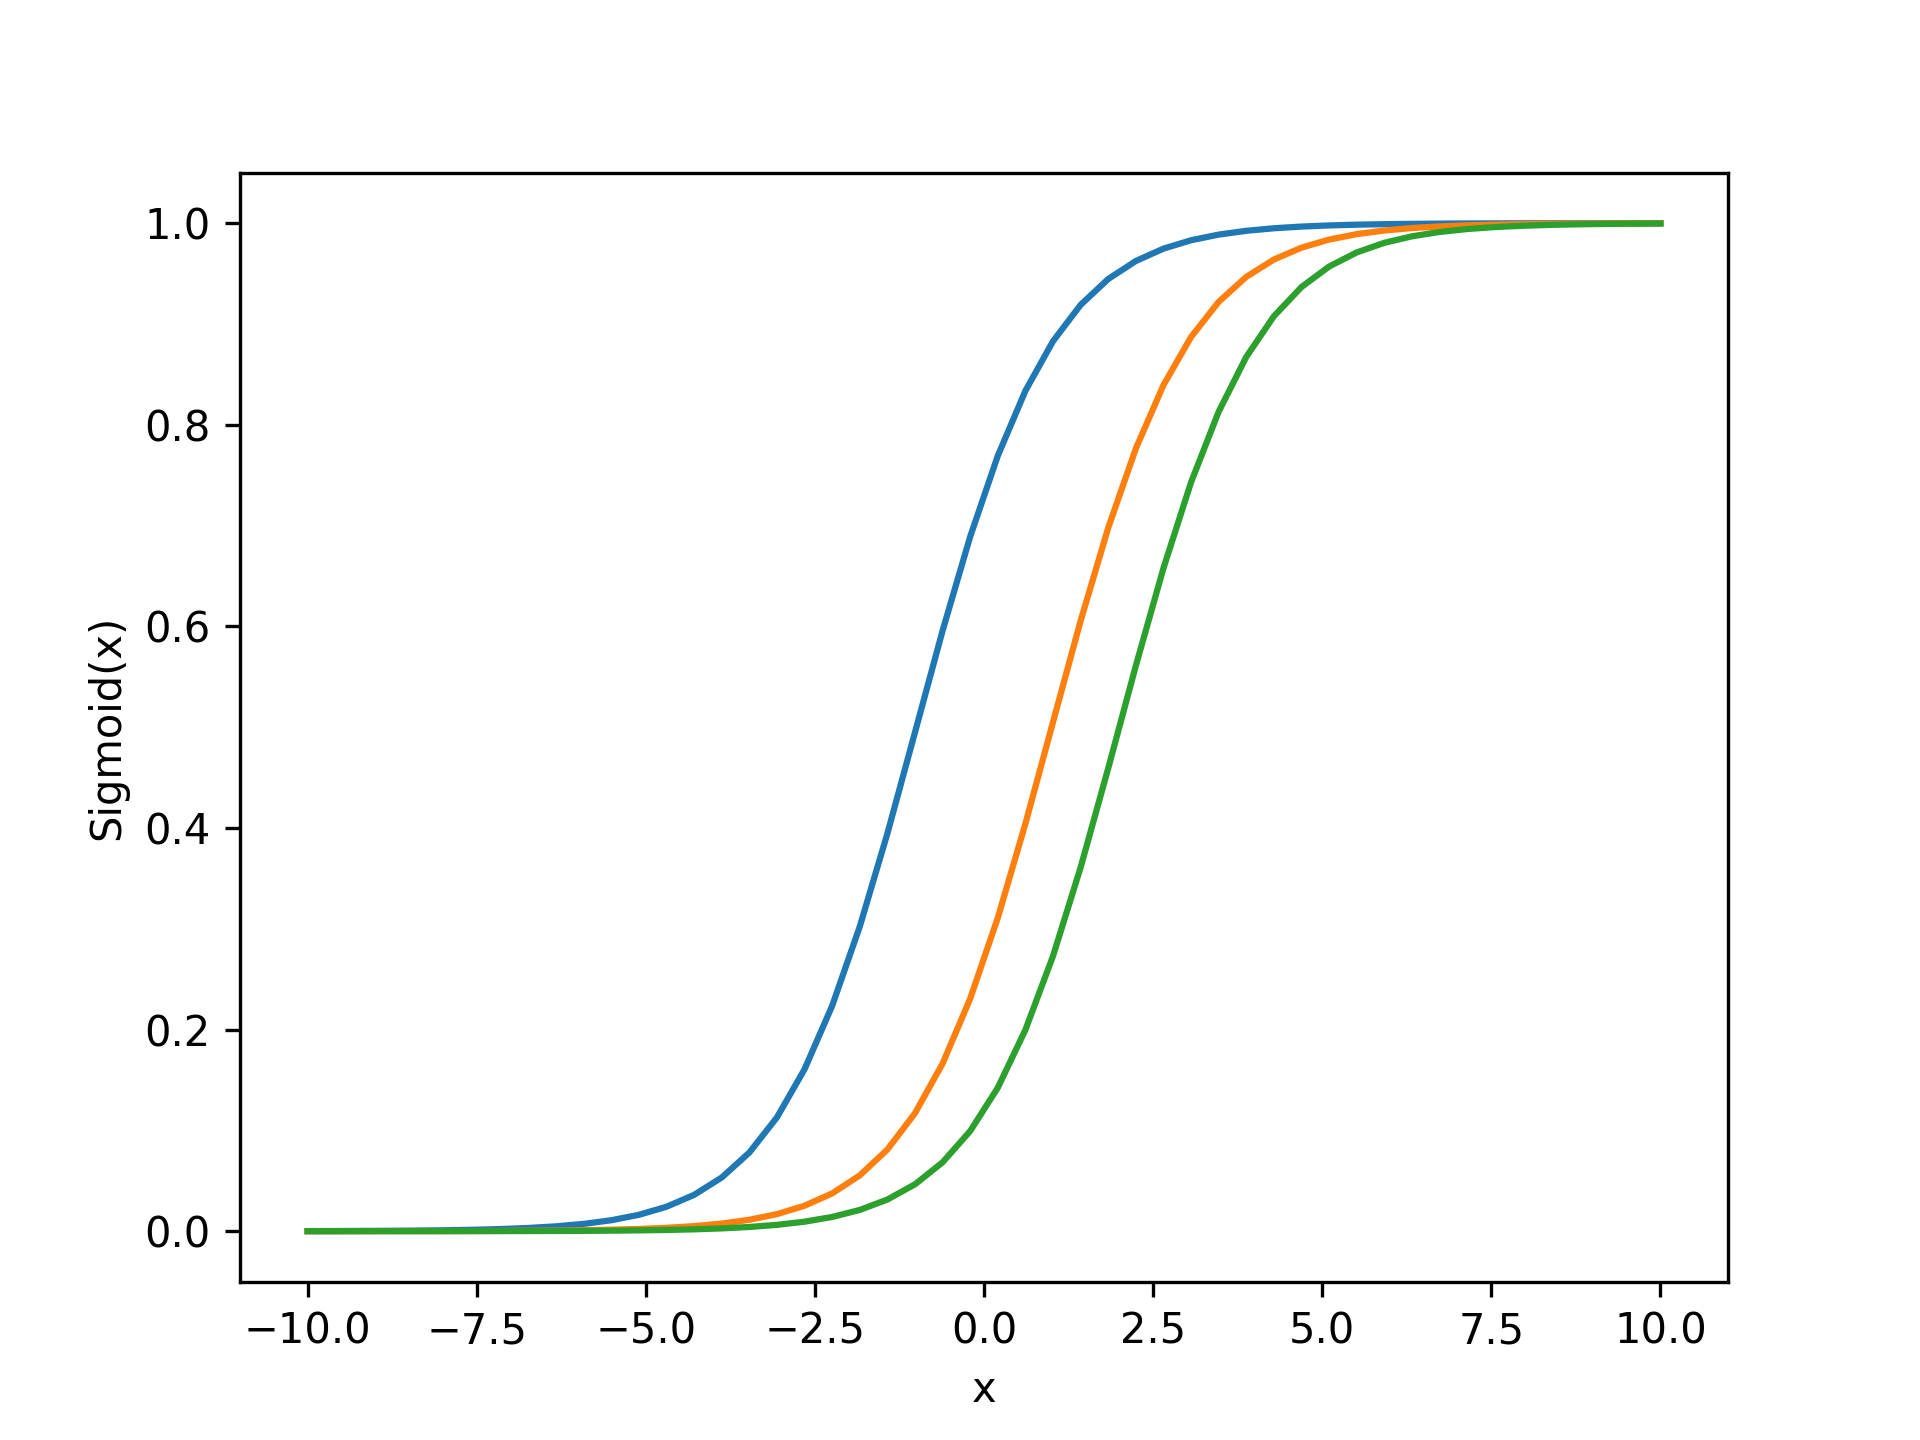
\includegraphics[width=8cm]{images/bias}
	\caption{Sigmoid function with same weights but different bias - [source:author]}
	\label{fig:sig_w_bias}
\end{figure}
The bias therefore is utilised to directly influence the result of the activation function and whether or not a certain neuron is activated or not. 
\subsubsection{Activation Function}
Activation functions introduce non-linearity characteristics to NN. This function is applied to the output of a neuron and decides whether or not a neuron is activated or not.\cite{activation} In combination with the descent gradient this function enables the NN to learn complex patterns within a training set. Originally the sigmoid function \cite{bp_basic} was used as activation function for NN but as of today multiple other functions like softmax, Tanh, ReLu emerged \cite{activation}.

\subsubsection{Phases} 
 Backpropagation follows an iterative process. At the beginning there is the feed forward pass. During this phase the input data is passed through all layers. Each hidden layer applies a linear function to create certain weights those outputs then are fed to the activation function. Depending on how many hidden layers are used within the NN the output of the activation function is used as input for the next neuron. At the end the predicted outputs by the model are compared with the actual outputs of the training data. This comparison is evaluated through a loss function. At this step the actual learning process of the model starts by calculating the gradient of the loss function considering the output of the NN. After that the back pass is initiated. Along this phase the gradients of each previous layer are multiplied with a local gradient and its weights which results in a gradient in respect to the layer's input. After receiving all gradients  based on the network's input data, all weights and biases are updated and optimised to reduce the result of the loss function. The steps forward pass, loss calculation, back pass, and the updates of weights and biases are repeated to improve the network in an iterative way. \cite{bp_basic} Figure \ref{fig:bp} demonstrates the logic of the backpropagation algorithm. Whereas \verb|wu| represents the updated weights after each iteration.  

\begin{figure}[H]
	\centering
		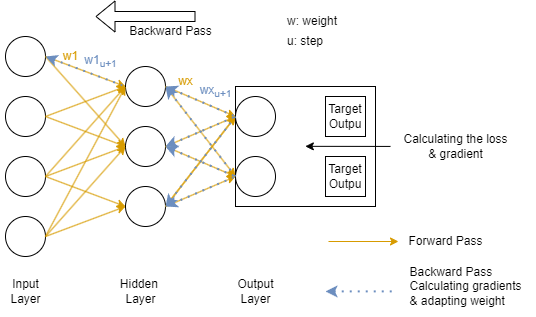
\includegraphics[width=14cm]{images/bp}
	\caption{Simplified logic of the backpropagation algorithmus - [source:\cite{bp_basic}]}
	\label{fig:bp}
\end{figure}
\section{The Models}
Both models CNN and RNN/LSTM can be used for time series forecasting. To create accurate prediction models a basic knowledge of the models functionalities are required. Therefore this section explains the components of each NN as well as the approaches those models follow. 

\subsection{LSTM}
\label{sec:lstm}
LSTM is a RNN and was invented by \cite{lstm_inventor} in 1997. Until today this NN is widley used for time series forecasting and provides reliable results for short as well as long term predictions \cite{rnn_moharm}. LSTM has so called memory cells which are responsible to store the state of data. Whenever information arrives at a memory cell its outcome is defined by refreshing the cell state with the newly arrived information. LSTM utilizes gates to control a cells state by either including or excluding information \cite{lstm_stock}. The gates are called: 
\begin{itemize}
\item input gate - data selection and storage for upcoming state
\item forget gate - data selection and storage which will not be used for the upcoming state
\item output gate - sets information within the state that is send to the output
\end{itemize}
Those gates are created by combining sigmoid functions. The results of these gates are values ranging from zero to one. A result of zero indicates the cell to not pass any information whereas values close to one indicate the cell to pass all information. 
The LSTM module or Repeating module consist of four NN layers which interact together as shown in Figure \ref{fig:lstm_rep_model}:
\begin{figure}[H]
	\centering
		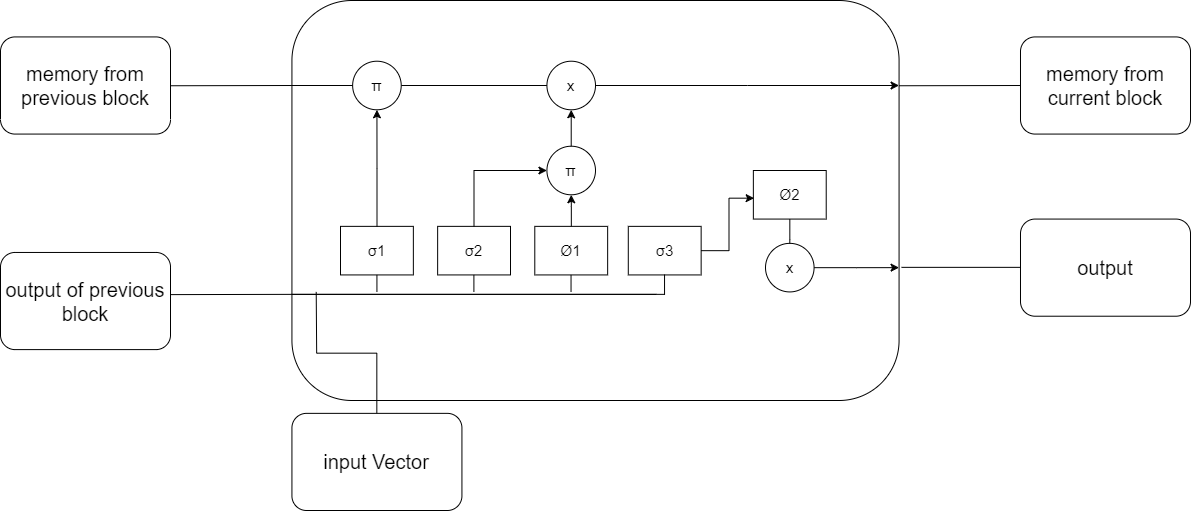
\includegraphics[width=14cm]{images/lstm_module}
	\caption{Repeating LSTM module - [source:\cite{lstm_module}]}
	\label{fig:lstm_rep_model}
\end{figure}
In total the repeating model has three gate activation functions which are named $\sigma_1$, $\sigma_2$,  $\sigma_3$ and shown in figure \ref{fig:lstm_rep_model}. Furthermore $\sigma_1$ and $\sigma_2$ act as output activation functions too. The cell state is illustrated using a blue line which starts at St-1 and indicates the previous memory block to St representing the current memory block. The amount of information that is passed is regulated by layer  $\sigma_1$ using the following function:
\begin{equation}
cf_t = \sigma_1 (W_cf * [O_t-1, x_t] + b_cf)
\cite{lstm_module}
\label{eq:eq_1}
\end{equation}
Furthermore two network layers are used to store new information to the cell state. Therefore sigmoid layer $\sigma_2$ chooses the values which are updated by utilising the following formula:
\begin{equation}
l_t = \sigma_2(W_1 *[O_t-1, x_t]+ b_l)
\cite{lstm_module}
\label{eq:eq_2}
\end{equation}
Layer $\phi_1$ or \verb|tanh| is created by using new candidate values. This layer outputs a  vector by utilzing the following formular: 
\begin{equation}
\widetilde{S}_t = tanh(W_s * [O_t-1, X_t] + b_s)
\cite{lstm_module}
\label{eq:eq_3}
\end{equation}
The last step includes combination of both states \ref{eq:eq_2} and \ref{eq:eq_3} which is added to the state. Also the state is reconditioned by applying: \cite{lstm_module}
\begin{equation}
S_t = cf_t * S_t1 + I_t * \widetilde{S}_t-1
\cite{lstm_module}
\label{eq:eq_4}
\end{equation}

The reason why a LSTM model is used for this purpose is that a standalone RNN is challenging to train due to its characteristics. As BP is used for RNNs, problems like vanishing-gradient can occur. The gradient in general can be understood as a computed value through all time steps which in the end used to update parameters of the RNN. The vanishing-gradient over time results in information decay. By implementing a LSTM module this problem can be solved. \cite{lstm_overcome_rnn_problem}

\subsubsection{Bidirectional LSTM}
Bidirectional LSTMs are able to look in both directions past and future. This is achieved by processing the available data into both directions. Therefore those models make use of bidirectional layers. Those layers split up the used neurons into two directions. \cite{bi_di_1} This provides more information to the network as the model is now capable of storing the forward state as well as the backward state, resulting in potentially more accurate results \cite{bi_di_2}. 

\subsection{CNN}
\label{sec:cnn}
CNNs follow the concept of NN consisting of multiple layers. The scope of application for this kind of network reaches from computer vision problems to time-series forecast modelling. Whereas data provided for image classification is structured in multi dimensional arrays (matrices), data used for time-series forecasting is provided via one dimensional arrays.\cite{cnn_intro} A CNN provides different types of layers. Those layer types are called Pooling Layer (PL), Fully Connected (FC), Convolution layer (CL) and flatten layer (FL). The connection of those layers are demonstrated in figure \ref{fig:cnn_struct}.
\begin{figure}[H]
	\centering
		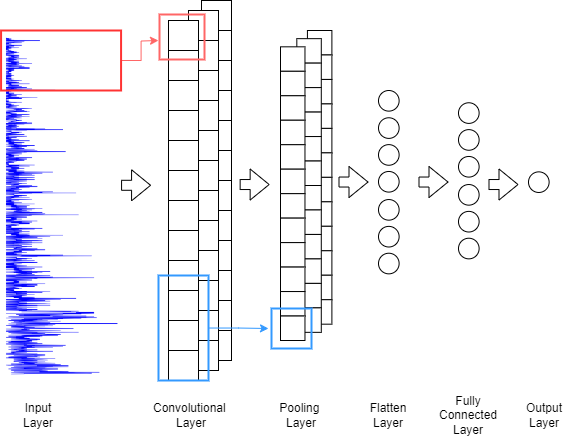
\includegraphics[width=10cm]{images/1d_cnn_model}
	\caption{One Dimensional CNN Structure - [source:\cite{cnn_vechicle}]}
	\label{fig:cnn_struct}
\end{figure}

CNN is based on convolution which is a linear operation that multiplies input data with convolution filters. Those filters which are also called kernels correlate to a set of weights \cite{cnn_vechicle}. The kernel values are created during the learning process and are optimised from the NN utilising BP. Furthermore this layer is utilised to detect features within the given one dimensional array. Those features are stored within a feature map and are calculated by applying convolutions on the input data. One crucial parameter to detect proper features is the size of the kernel. The kernel size can be understood as a number of weights that are multiplied with the input data. After each multiplication the sequence is shifted along the input data. Each shift during this process produces one output which is stored in the feature map. The following example demonstrates how this process is done:\cite{1d_cnn}
\begin{lstlisting}
Input Data: [4,7,10,43,20,10] e.g. number of bookings per day. 
Kernel: [0.5,0.25,0.2] Kernel size = 3
1st Multiplication: 4*0.5 + 7*0.25 + 10*0.2 = 5.75
2nd Multiplication: 7*0.5 + 10*0.25 + 43*0.2 = 14.6
...
Output sequence [5.75, 14.6, ...]
\end{lstlisting}
The second operation that is used within the CNN is called activation function. This non-linear function is utilized to detect complex relationships between variables and are applied onto the feature map. As of today multiple functions like ReLU, sigmoid and softmax can be used as activation functions \cite{cnn_basic3}.

The pooling layer as shown in figure \ref{fig:cnn_struct} is deployed within a NN to diminish the size of feature maps. To reduce the size pooling operations like average pooling, max pooling or sum pooling can be applied. Applying one of those operations results in less computational effort.\cite{cnn_basic}

%The activation function is also part of the fully connected layer. This layer applies the activation function onto the feature map and enables the model in combination with BP to learn complex connections between features. Furthermore this layer operates on the already flatten feature map and outputs a 2d vector.\cite{1d_cnn}

The flatten layer transforms two dimensional input data into one dimensional input vectors. Its output is used to provide values to the fully connected layer. Overfitting can be caused whenever all features are used in the flatten layer. Therefore a dropout layer can be set in place.****CITEHERE**** This layer cancels out neurons during the training process of a NN which reduces the model's size. 

\section{Loss Function}
\label{sec:loss_func}
The loss function is one crucial element as it evaluates the accuracy of the produced outputs from a NN. This is achieved by calculating the difference between the predicted value and the actual value provided by the test dataset. Supervised learning deals with two different problems which is either a classification problem e.g. is the animal on the picture a cat or with regression problems like predicting future bookings. Both of those problems use a different loss function.\cite{loss_func} As this section focuses on solving a regression problem a brief overview of available loss functions and their characteristics are given. 

\begin{table*}[htbp]
	\centering
		\begin{tabularx}{\textwidth}{|l|X|}
		\hline
		\rowcolor[gray]{0.9}
		Function & Characteristics \\
		\hline
		Square loss &Sensitive to outliers (Model tends to focus on those outliers whereas accuracy for normal values decline)\\
		 \hline
		Absolute loss & Outliers do not influence the model as  severe as compared to square loss.  \\
		\hline
		Huber & Combination of square loss and absolute loss - Outliers do not influence the accuracy of results and learning from smaller errors can still be done in a efficient way  \\
		\hline
		Log-cosh & Similar to Huber when it comes to its characteristics. Does not handle large errors well because the gradient tends to stay constant. \\
		\hline
		Quantile loss & Extends absolute loss and provides prediction intervals. Utilising a punishment system for overestimated and underestimated samples. \\
		\hline
		$\epsilon$-insensitive & Focuses on samples with large prediction errors \\
		\hline	
		\end{tabularx}
	\label{tab:loss_function}
	\caption{Loss functions and their characteristics - [source:\cite{loss_func}]}
\end{table*}

By looking at the characteristics of the augmented data set shown in figure \ref{fig:augmented_data} it is clear to see that the dataset itself has got outliers repeating themselves every year. To avoid a strong focus on those peaks both models are initially trained utilising the Adam loss function.

\section{Optimise Function}
\label{sec:optimize_func}
To optimise the parameters of a NN an optimiser function is required. This function updates parameters like weights based on the results provided by the loss function \cite{optimizer}. Since both NNs described in this section make use of BP for their training. A literature review was conducted to figure out which optimiser is keen to deliver the most accurate results. By inspecting the advantages and disadvantages proposed by these works \cite{optimizer}\cite{otimizer_1}\cite{optimizer_2} it turns out that the algorithm Adam is a valid choice. This algorithm is characterised by achieving faster convergence compared to other algorithms. Furthermore Adam provides a decent performance for datasets with meager features.

\section{Implementation}
\label{sec:implementation}
Both models follow the same workflow when it comes to their implementation. The workflow is highlighted in figure \ref{fig:workflow}:

\begin{figure}[H]
	\centering
		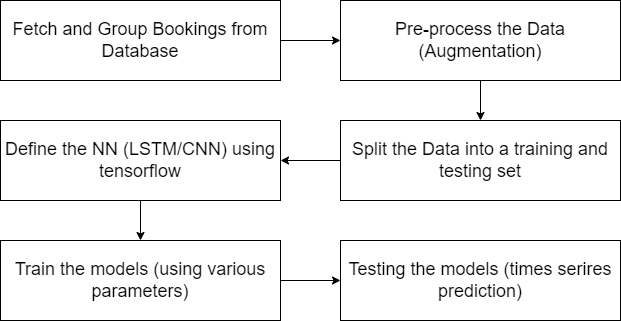
\includegraphics[width=12cm]{images/workflow_imp}
	\caption{Workflow of the implementation - [source:[author]]}
	\label{fig:workflow}
\end{figure}

As each booking correlates to one entry within the database table those entries need to be grouped on a daily basis. Therefore the following sql query is executed: 
\begin{lstlisting}
import mysql.connector
import logging
import pandas as pd

def get_booking_data():

       sql = ("SELECT count(taskFrom_time) as bookings, date(taskFrom_time) "
           "from bookings_2 "
           "WHERE date(taskFrom_time) <= DATE('2023-05-01') and date(taskFrom_time) >= 			DATE('2017-01-01') "
           "Group By date(taskFrom_time) order by date(taskFrom_time) asc")

    res = pd.read_sql(sql, connection)
    return res
\end{lstlisting}

Once the data is retrieved from the database it is directly converted to a \verb|pandas dataframe|. As mentioned in chapter \ref{sec:data_aug} data augmentation is necessary to compensate the lack of data during Covid19. Corresponding to the workflow described in figure \ref{fig:workflow} the data now needs to be separated into a training and test set. The training set is used to train the model whereas the test set is used to evaluate how the trained model performs. Therefore the trained model is used to predict the values for timestamps used in the test set. By reviewing other scientific works that deal with time series forecasting \cite{1d_cnn}\cite{cnn_vechicle}\cite{cnn_intro}\cite{lstm_overcome_rnn_problem}\cite{lstm_module}\cite{lstm_stock} the most accurate results are achieved by using ranges from 80 \% to 90 \% for training and depending on the range for training data a range of 20 \% to 10 \% for test data are recommended. The initial split used for both models correlates to 90\% training data to 10 \% test data as visualised in figure \ref{fig:training_test}. Therefore the following code is applied to split the data:
\begin{lstlisting}
training_end = pd.to_datetime('2022-10-31')
#total range 2017-01-01 - 2023-05-31 = 2342 days
train = df[:training_end]
# 2017-01-01 - 2022-10-31 = 2129 days ~ 90%
test = df[training_end:]
# 2022-10-31 - 2023-05-01 = 213 days ~ 10%
\end{lstlisting}
\begin{figure}[H]
	\centering
		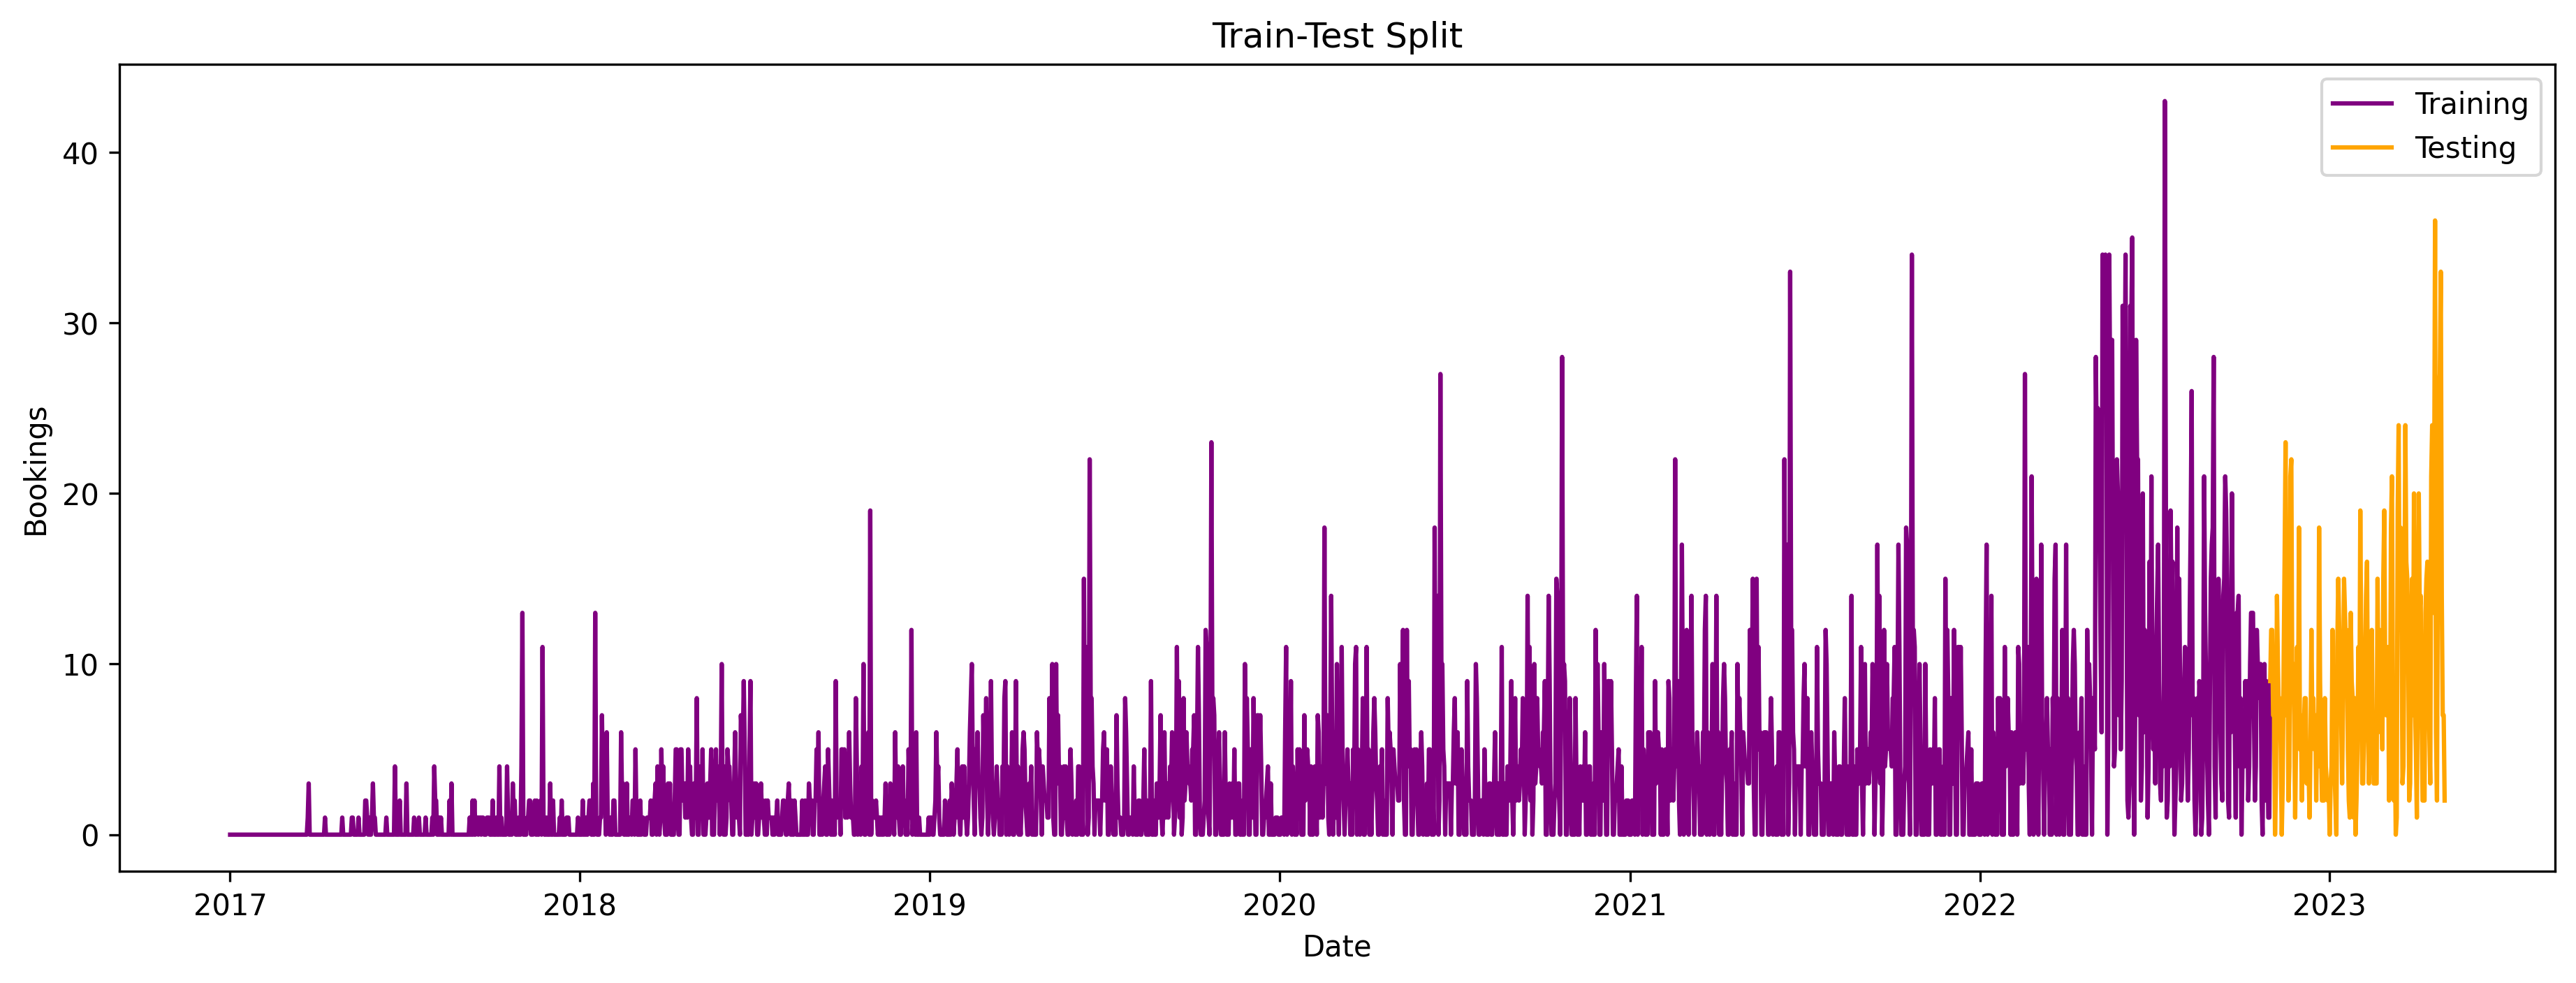
\includegraphics[width=14cm]{images/training_test}
	\caption{Visualised Training-Test split (90\%-10\%) - [source:[author]]}
	\label{fig:training_test}
\end{figure}
With the training and test data in place the next step is to implement both models (LSTM, CNN) by utilising the \verb|tensorflow| library. To reduce computation costs and to increase training efficiency the training data is further processed in the following way:
\begin{lstlisting}
WINDOW = 20
bookings_training_90 = tf.data.Dataset.from_tensor_slices(train.values)
bookings_training_90 = bookings_training_90.window(WINDOW + 1, shift=1, drop_remainder=True)
bookings_training_90 = bookings_training_90.flat_map(lambda x: x.batch(WINDOW + 1))
bookings_training_90 = bookings_training_90.map(lambda x: (x[:-1], x[-1]))
\end{lstlisting}
On line 2 the code above transforms the training data into a \verb|TensorSliceDataset|. This data format grants access to tensorflow's data API which supports the user to manipulate the data further. As this is time series data the model itself is fed with data limited to certain ranges. The constant \verb|WINDOW| indicates how many consecutive timestamps are used as input to predict the next time step. The function \verb|flat.map()| is now used to flatten the dataset. As \verb|from_tensor_slices()| creates a single tensor for each entry in a window \verb|flat.map()| combines those windows to a single tensor holding the windowed data. Line 5 prepares the data and splits each window into features and target values. As the learning process described in section \ref{sec:bp} involves multiple inputs that are used to predict one output the \verb|.map()| function prepares each windowed tensor by using the interval from \verb|x to x-1| to predict \verb|x-1|.
Both models LSTM and CNN are trained with the prepared data explained in during this section. 

\subsection{Implementation of LSTM}
The code itself required to setup a LSTM model only requires a few input parameters. Therefore it is crucial to understand the meaning behind the input parameters as well as how they can influence the training results of the model itself. The following code is used to initialise the model:   
\begin{lstlisting}
#define the model
lstm_booking_prediction_model = Sequential([
    Lambda(lambda x: tf.expand_dims(x, axis=-1), input_shape=[WINDOW]),
    Bidirectional(LSTM(128, activation='tanh',recurrent_activation='sigmoid' )),
    Dense(units=128, activation='relu'),
    Dropout(0.4),
    Dense(1)
	])
\end{lstlisting}
When utilising LSTM for time series predictions a certain input format for data is needed. Therefore the Lambda function on line 3 is required to reshape the dimension of the used input data. 
\verb|Bidirectional()|\footnote{\label{tf_fn}\url{https://www.tensorflow.org/api_docs/python/tf/keras/}} actually represents a wrapper for the actual layer used for this model. In this case it is holding additional states and is used to create a Bi-LSTM model as described in section \ref{sec:lstm}. \newline
\verb|LSTM()|\textsuperscript{\ref{tf_fn}} contains actual logic as described in section \ref{sec:lstm}. Moreover the parameter \verb|unit=128|\textsuperscript{\ref{tf_fn}} can be understood as the number of neurons used within this layer. Furthermore this model offers different kinds of activation functions. By default the hyperbolic tangent (tanh)\cite{tanh} is used. Whereas the \verb|recurrent_activation| defines which functions are used for the actual gates within the module as described in section \ref{sec:lstm}. Whenever creating a stacked LSTM model, which means it makes use of at least two LSTM layers the parameter \verb|return_sequences| must be set to true. Otherwise the layer's output results in a 2d tensor output which only provides information about the last timestep. This format cannot be passed on to the next LSTM layer. \newline
\verb|Dense()| is used to implement fully connected layers whereas \verb|units| correlate to the amount of neurons used for this layer. The last \verb|dense(1)| layer is used to reduce the number of outputs to 1. The way this layer works is explained in section \ref{sec:cnn}. Additionally the model needs to be compiled. Therefore the following code is required: 
\begin{lstlisting}
#compile the model 
lstm_booking_prediction_model.compile(
    loss=Huber(),
    optimizer=Adam(),
    metrics=['mae']
	)
\end{lstlisting}
The parameter \verb|loss| sets the loss function which is utilised to evaluate the models performance. The reason why \verb|Huber| is used is explained in section \ref{sec:loss_func}. Futhermore the model also requires an optimising algorithm. This algorithm is assigned by using the \verb|optimizer| parameter. Due to the results the literature review explained in section \ref{sec:optimize_func} Adam turned out to be the most promising candidate for this purpose. To observe the capability of learning of a given model the metric mean absolute error (MEA) can be used. 

The next step is to start the training of the model as demonstrated below:
\begin{lstlisting}
#start to train the model
lstm_history = lstm_booking_prediction_model.fit(
    bookings_training_90,
    epochs=100,
    verbose=1,
    use_multiprocessing=True
	)
\end{lstlisting}
The function \verb|fit()| requires parameters like the data used for training (\verb|bookings_training_90|) as well as how many epochs are processed. One \verb|epoch| covers the process of iterating through the entire training dataset and performing forward and backward propagation as well as updating the model's parameters based on the chosen optimisation algorithm.
\newline
When training the model using the initial parameters described during this chapter the following results are achieved:
\begin{figure}[H]
	\centering
		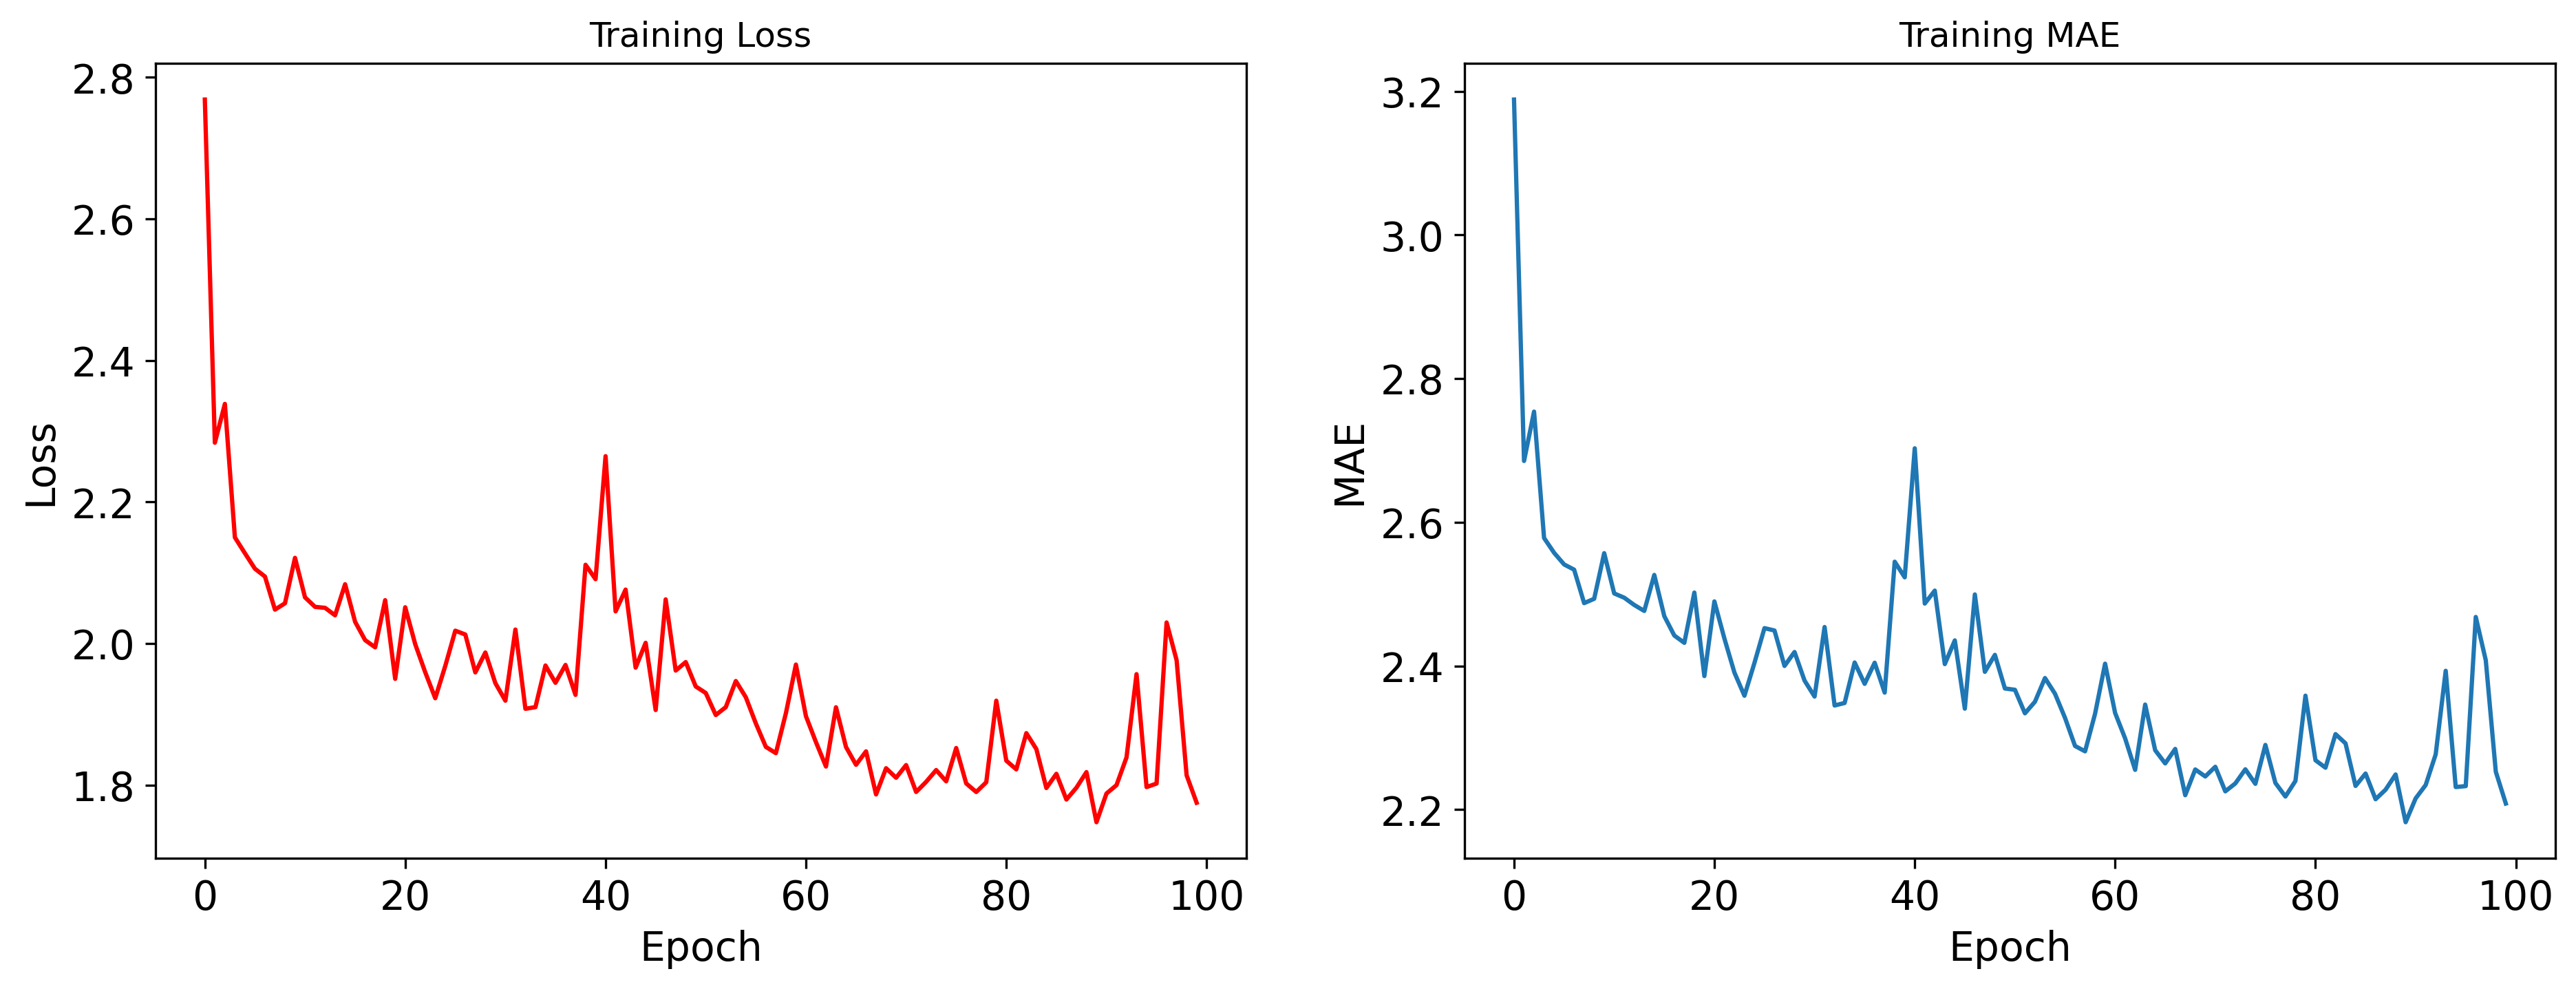
\includegraphics[width=14cm]{images/lstm_1_paper_training}
	\caption{Decrease of MAE and Trainig loss for 100 epochs - [source:[author]]}
	\label{fig:training_test}
\end{figure}
The training loss in general indicates the performance of the model based on the training set. It is generated through the output of the applied loss function. Low values basically mean that the model is able to catch up patterns within the training set but could also indicate overfitting. This causes the model to just memorize the training set rather than learning actual patterns. Furthermore the loss indicates the amount of required epochs for the model to learn. Whenever the loss stalls or is starting to increase again the training should be stopped. The MAE is another metric to observe the ability of the model to learn. The MAE is obtained by calculating the mean of actual values minus the predicted values. This result is divided by the number of observations.\cite{mae} Similar to the training loss a lower value indicates the performance of the model but the MAE needs to be interpreted in context with the range the predictions are made for. For example a MAE of 1 for predictions made in ranges between 1-2 is interpreted as poor performance, whereas a MAE of 100 for predictions made in a range between 100.000 and 1.000.000 indicates a proper result.

\begin{figure}[H]
	\centering
		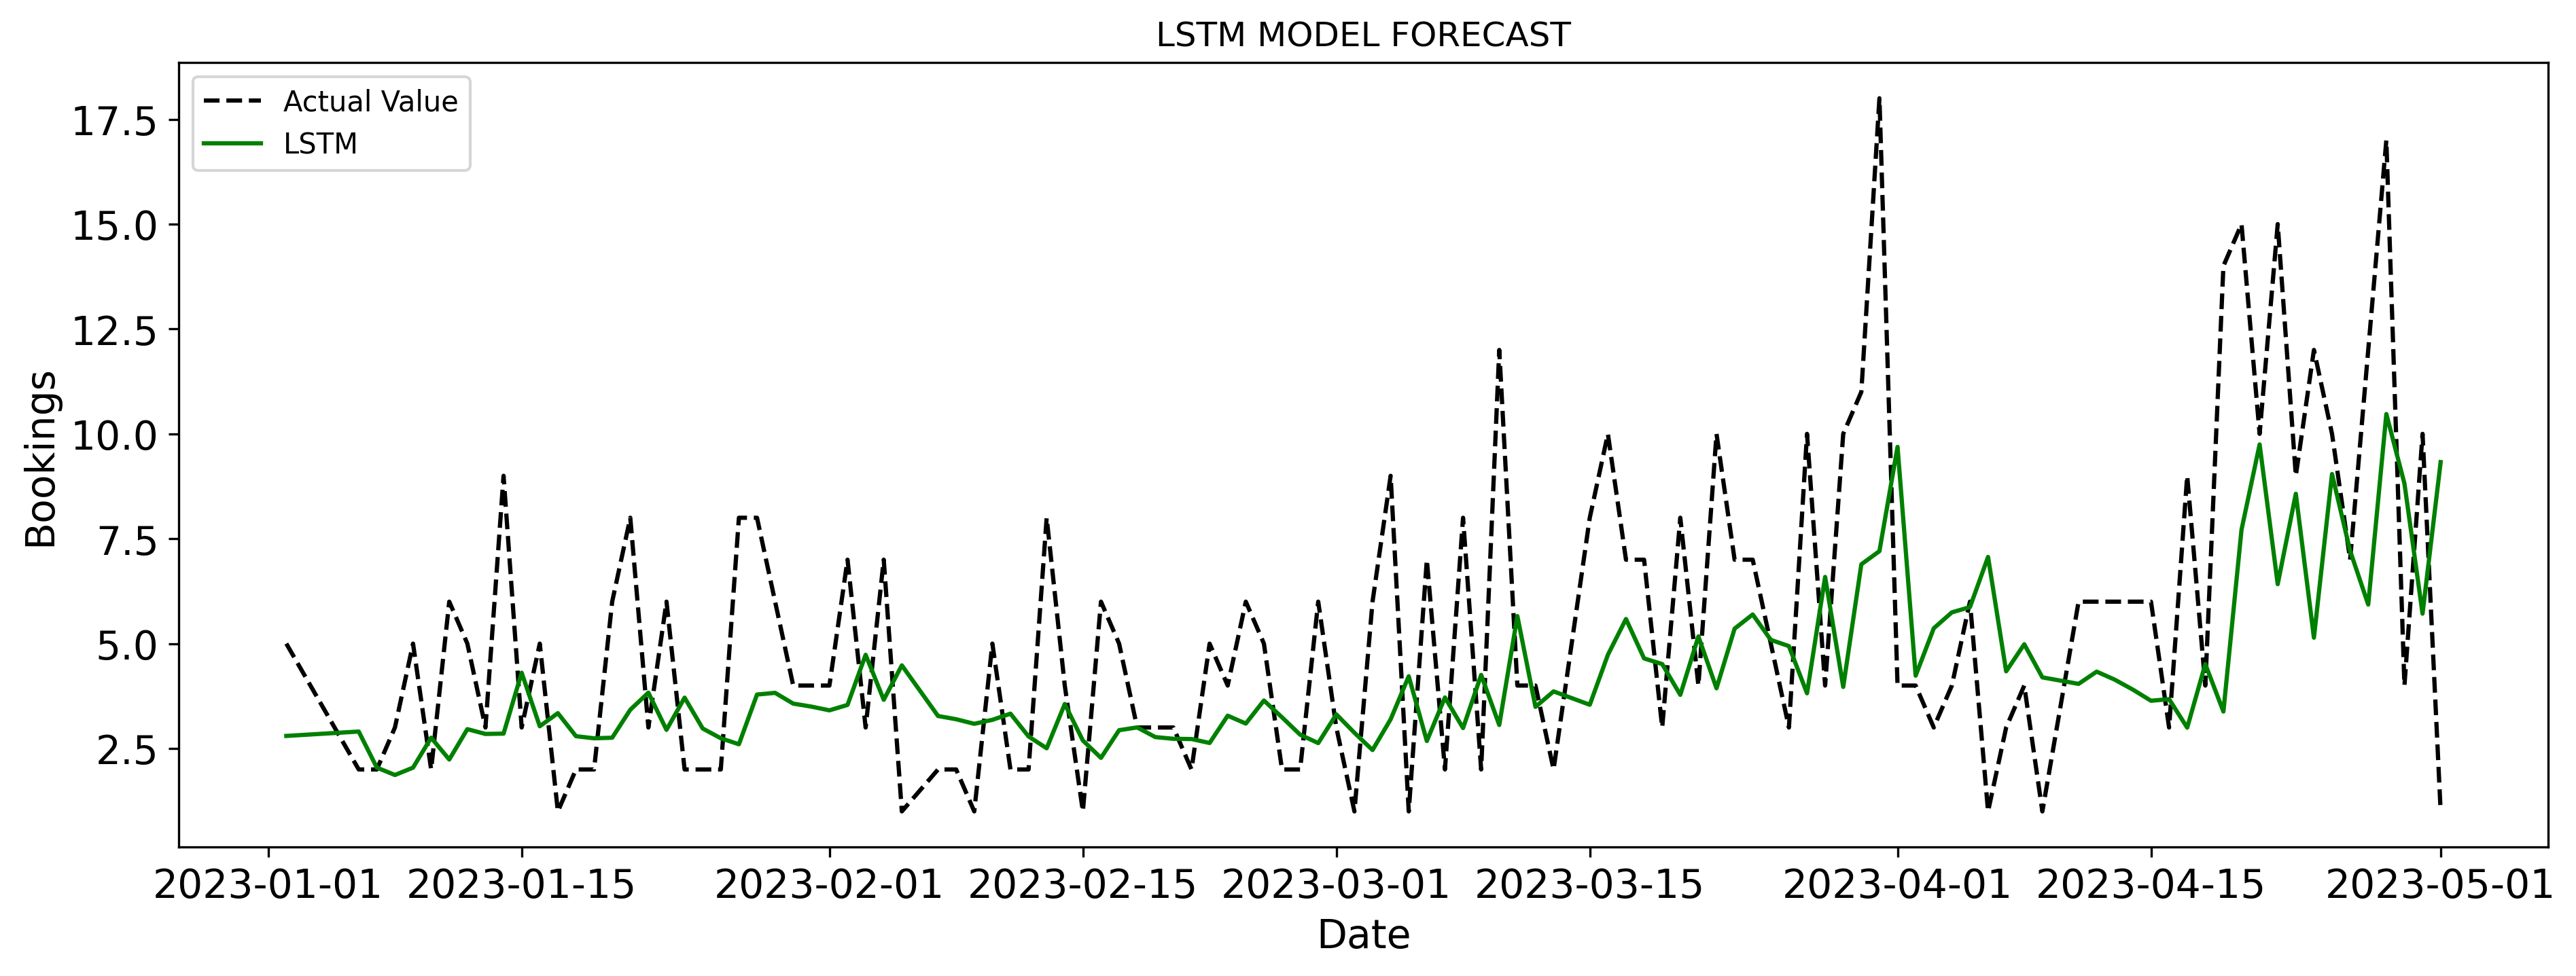
\includegraphics[width=14cm]{images/paper_1_lstm_1_prediction}
	\caption{Predictions on test set from 01-01-203 to 01-05-2023 - [source:[author]]}
	\label{fig:lstm_1_training_test}
\end{figure}
By looking at figure \ref{fig:lstm_1_training_test} it is clear to see that the model's performance in terms of accuracy is insufficient. Investigating the training loss and MAE shows that the final MAE of around 0.5 is acceptable in context of the prediction range ranging from 1 to 17. This indicates that the model tends to overfitting as the final training loss is low as well. Section \ref{sec:improving} investigates strategies on how to improve the model's performance.

\subsection{Implementation of CNN}
Similar to the implementation of LSTM the implementation of a CNN does not require much code. Furthermore some parts of the code use the same parameters. Those parameters are not explained again. To initialise a CNN model the following code is required: 

 \begin{lstlisting}
#define the model 
    Lambda(lambda x: tf.expand_dims(x, axis=-1), input_shape=[WINDOW]),
    Conv1D(filters=128, kernel_size=10, strides=1,
           padding='causal', activation='relu'),
    Conv1D(filters=128, kernel_size=10, strides=1,
           padding='causal', activation='relu'),
    GlobalAveragePooling1D(),
    Flatten(),
    Dropout(0.4),
    Dense(1)
\end{lstlisting}
\verb|Conv1D()| is used to add one 1d CL to the model. Those layers work as described in section \ref{sec:cnn}.  The \verb|filter| parameter is equivalent to the number of neurons this layer is going to use. Furthermore the kernel's size as explained in section \ref{sec:cnn} is determined by the parameter \verb|kernel_size|.
The only difference left in comparison to the LSTM layer is the FL describe in section \ref{sec:cnn}. This layer is added by utilising the \verb|Flatten()| parameter. When it comes to compiling and fitting the model the CNN makes use of  \verb|Huber()| for its loss function and \verb|Adam()| for its optimisation function contrary to the implementation of the LSTM model. Furthermore both models are initially using 100 epochs for their first training. \newline

The first training results produced by the CNN model look the following: 

\begin{figure}[H]
	\centering
		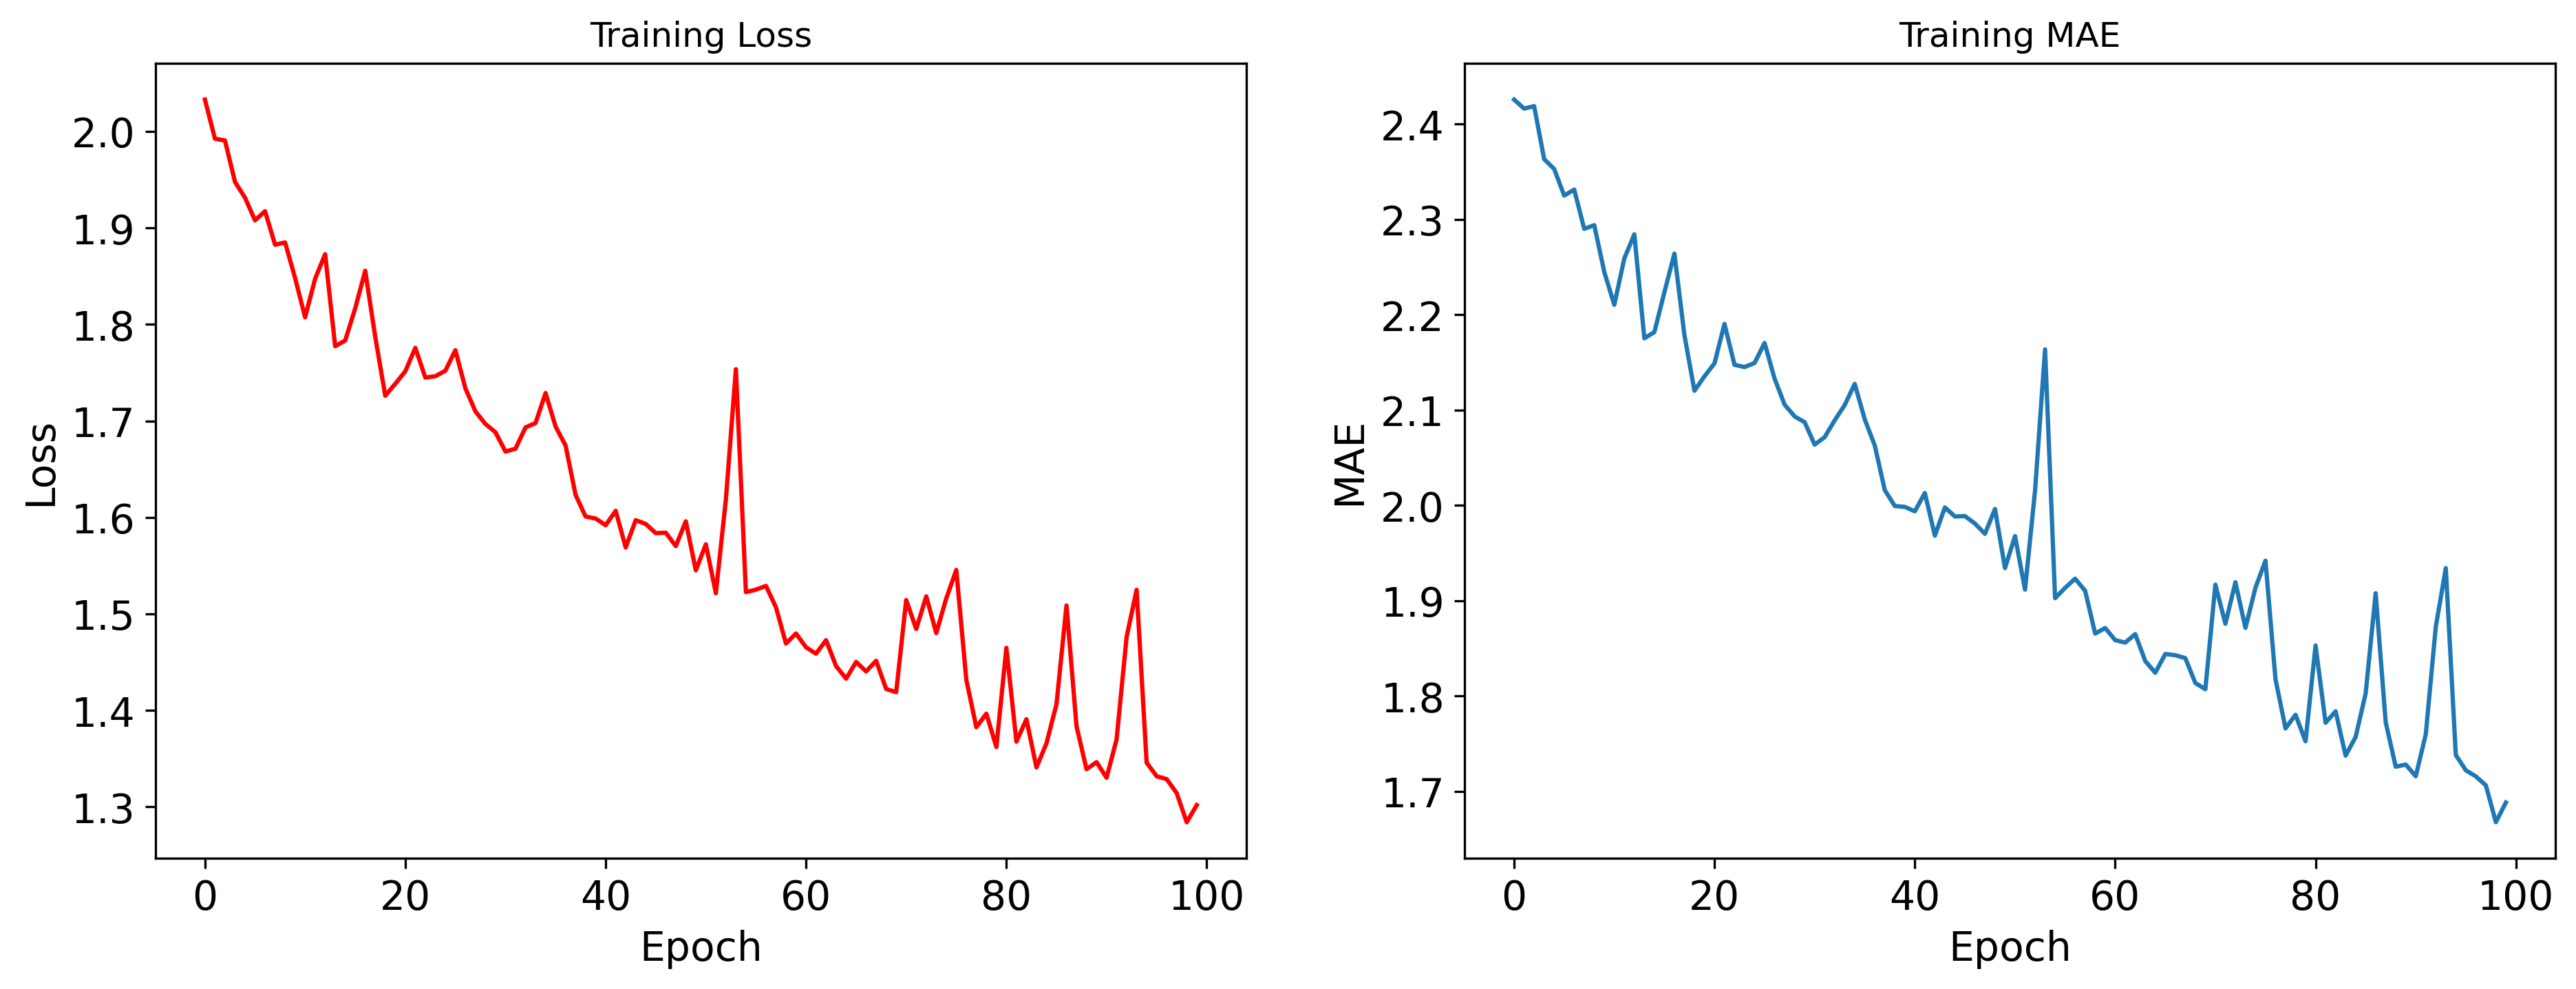
\includegraphics[width=14cm]{images/cnn_model_1_loss}
	\caption{Decrease of MAE and Trainig Loss for 100 epochs - [source:[author]]}
	\label{fig:training_test_cnn}
\end{figure}
When analysing the metrics highlighted in figure \ref{fig:training_test_cnn} it is clear to see that both the training loss and the MAE are still very high after 100 epochs. This indicates that the model needs to be trained utilising more epochs. The results of the training loss as well as the MAE are reflected also in the actual predictions made on the test set.

\begin{figure}[H]
	\centering
		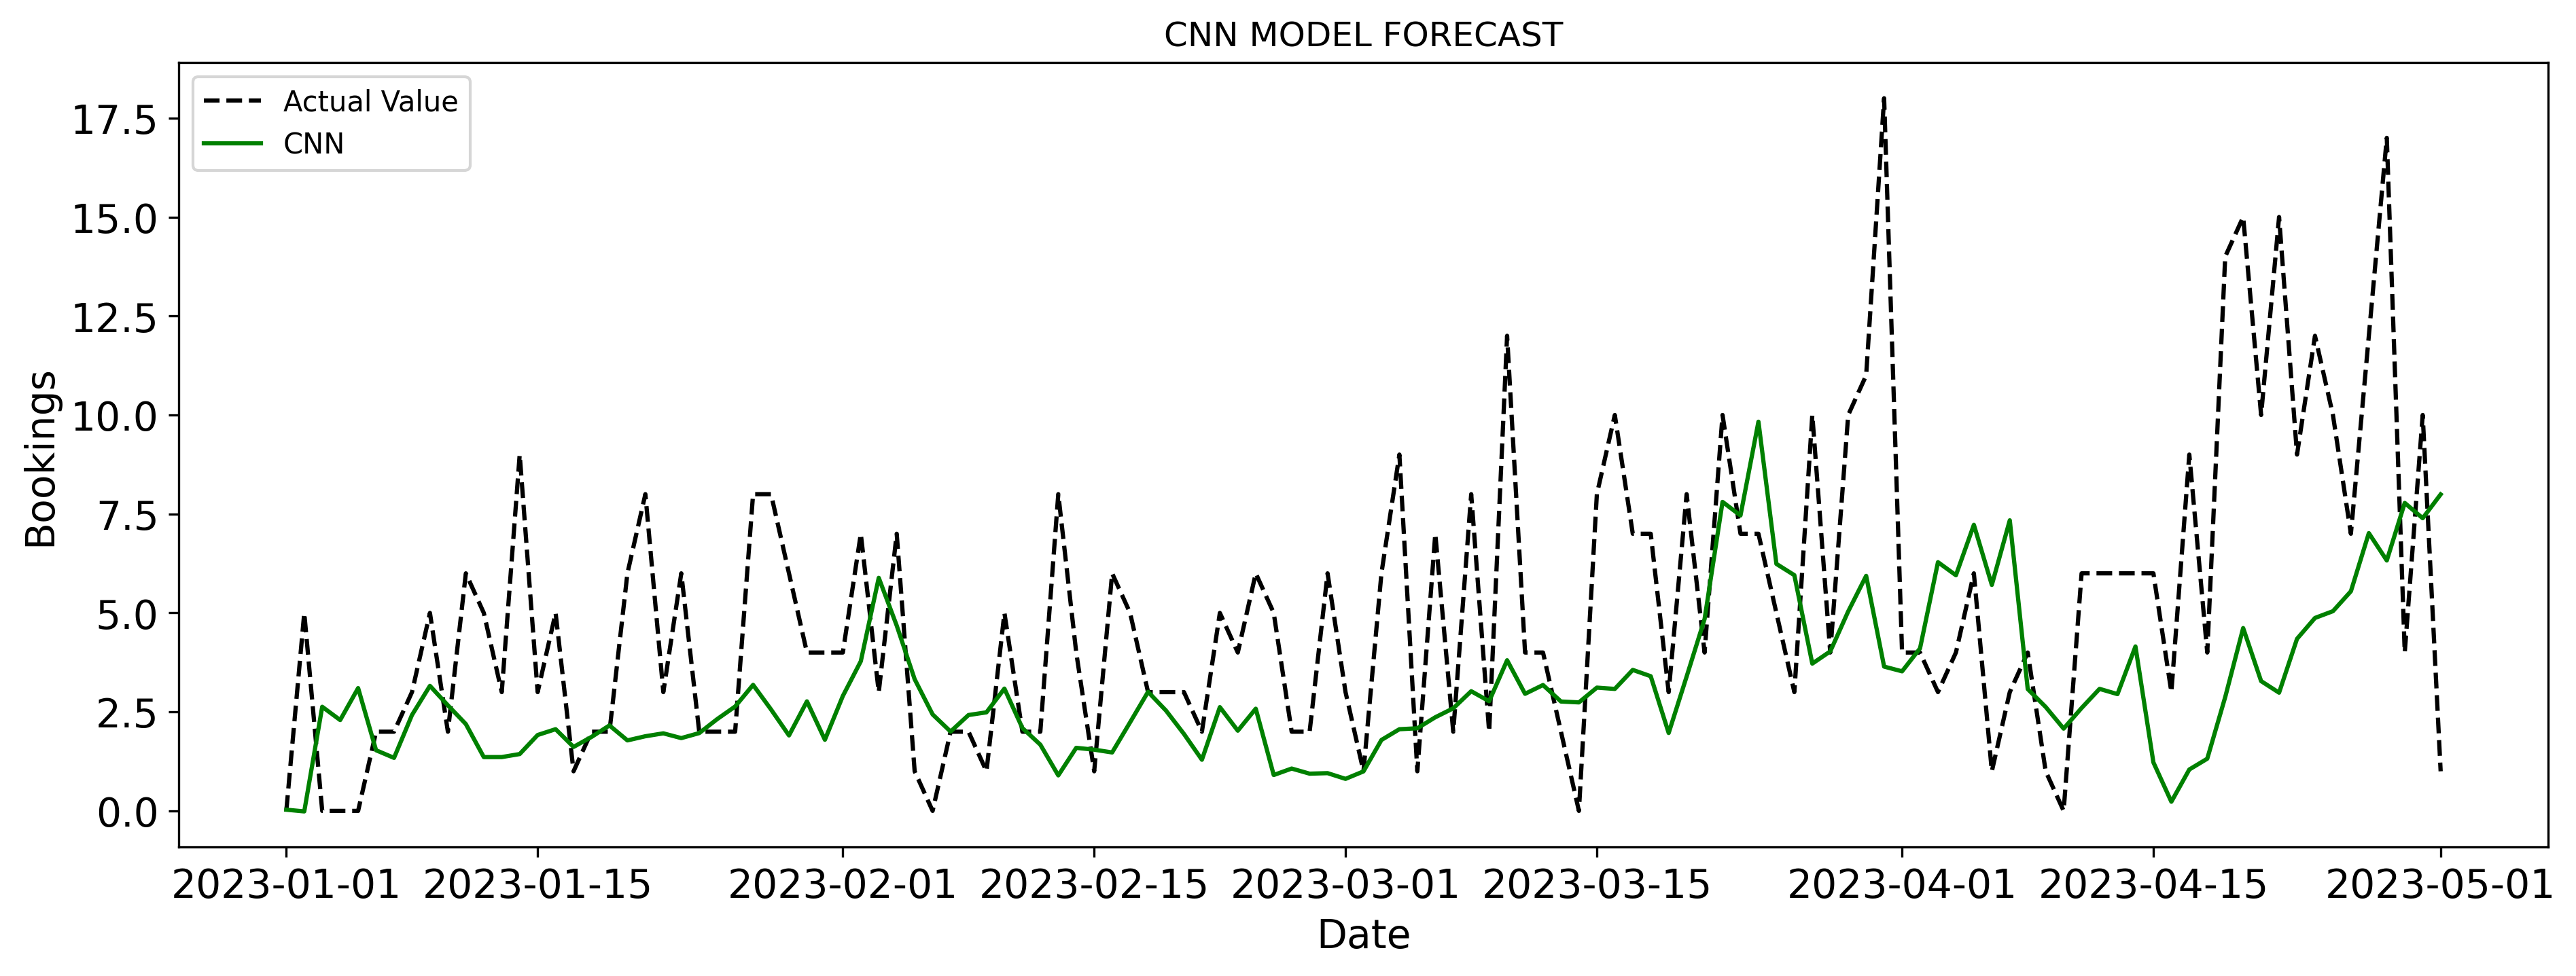
\includegraphics[width=14cm]{images/cnn_1_prediction}
	\caption{Predictions on test set from 01-01-203 to 01-05-2023 - [source:[author]]}
	\label{fig:cnn_1_training_test}
\end{figure}
By looking at figure \ref{fig:cnn_1_training_test} it is clear to see that the model's performance is poor. During it is training the model was not capable of obtaining the training's set characteristics. Strategies on how to potentially improve the models accuracy are discussed in section \ref{sec:improving}.

\section{Improving the models}
\label{sec:improving}
There are several strategies that can be followed in order to improve a model's performance. One option is to enhance the data preprocessing. Therefore the available data set is normalised. One approach that can be utilised is Min-Max Normalisation \cite{min_max}. Following this approach the original data is brought into a range from values between 0 and 1 by keeping the actual ratio of the test and training data. 
Another approach is called feature engineering \cite{feature_eng}. Following this strategy further features are extracted from the available dataset. This process results in a multivariate prediction model \cite{multi}.
Additional possibilities to enhance a model's performance is to change its architecture. This implies methods like utilising multiple \verb|Conv1D| layers or stacking several LSTM layers. Applying this approach leads to more complex models which might improve a NN's ability to find patterns within the available dataset. Similar to this approach the tuning of a model's parameters is also called hyperparameter tuning.  This method applies different configurations of parameters to train the model and compares their results. Looking at the implementation of the LSTM  and CNN model described in section \ref{sec:implementation} parameters like \verb|epochs|, \verb|window|, \verb|units|(LSTM) or \verb|filters|(CNN), and \verb|Dropout|. As there is no model that fits all purposes those parameters are updated during an iterative process. \newline
One of the approaches to increase the model's performance in this section is a combination of changing the architecture of both models as well as changing their hyper parameters. 

\subsection{Adapting the Architecture and Hyperparameter tuning}
\label{sec:hyper}
This section proposes various configurations that are applied to both models in order to increase their accuracy. Therefore table \ref{tab:models} lists the various combinations used to train the models.

\newsavebox{\codebox} % For saving code in the first row
\newsavebox{\codeboxtwo} % For saving code in the second row
\newsavebox{\codeboxthree} % lstm 3
\newsavebox{\codeboxfour} % cnn 1
\newsavebox{\codeboxfive} % cnn 2

\newsavebox{\codeboxsix} % cnn 3

\begin{lrbox}{\codeboxsix} % Start saving into \codebox lstm1
\begin{lstlisting}[numbers=none, basicstyle=\tiny, numbersep=0pt, xleftmargin=0pt, xrightmargin=0pt, backgroundcolor=\color{white}]
Conv1D(filters=256, kernel_size=3, strides=1, 
	   padding='causal', activation='relu')
BatchNormalization()
Conv1D(filters=256, kernel_size=3, strides=1,
	   padding='causal',activation='relu')
BatchNormalization()
Conv1D(filters=256, kernel_size=3, strides=1, 
	   padding='causal', activation='relu')
BatchNormalization()
Flatten()
Dropout(0.4)
Dense(1)
\end{lstlisting}
\end{lrbox} % Stop saving into \codebox



\begin{lrbox}{\codeboxfive} % Start saving into \codebox lstm1
\begin{lstlisting}[numbers=none, basicstyle=\tiny, numbersep=0pt, xleftmargin=0pt, xrightmargin=0pt, backgroundcolor=\color{white}]
Conv1D(filters=64, kernel_size=10, strides=1,
    padding='causal', activation='relu'),
Dropout(0.2),
Conv1D(filters=64, kernel_size=10, strides=1,
    padding='causal', activation='relu'),
Dropout(0.2),
Conv1D(filters=32, kernel_size=10, strides=1,
    padding='causal', activation='relu'),
GlobalAveragePooling1D(),
Flatten(),
Dropout(0.1),
Dense(1)
\end{lstlisting}
\end{lrbox} % Stop saving into \codebox


\begin{lrbox}{\codeboxfour} % Start saving into \codebox lstm1
\begin{lstlisting}[numbers=none, basicstyle=\tiny, numbersep=0pt, xleftmargin=0pt, xrightmargin=0pt, backgroundcolor=\color{white}]
Conv1D(filters=256, kernel_size=3, strides=1,
       padding='causal', activation='relu')
Conv1D(filters=256, kernel_size=3, strides=1,
       padding='causal', activation='relu')
GlobalAveragePooling1D()
Flatten()
Dropout(0.4)
Dense(1)
\end{lstlisting}
\end{lrbox} % Stop saving into \codebox

\begin{lrbox}{\codebox} % Start saving into \codebox lstm1
\begin{lstlisting}[numbers=none, basicstyle=\tiny, numbersep=0pt, xleftmargin=0pt, xrightmargin=0pt, backgroundcolor=\color{white}]
Bidirectional(LSTM(units = 80,
 	return_sequences=False,activation="relu")),
Dropout(0.2),
Dense(1)
\end{lstlisting}
\end{lrbox} % Stop saving into \codebox


\begin{lrbox}{\codeboxtwo} % Start saving into \codeboxtwo lstm2
\begin{lstlisting}[numbers=none, basicstyle=\tiny, numbersep=0pt, xleftmargin=0pt, xrightmargin=0pt, backgroundcolor=\color{white}]
Bidirectional(LSTM(units = 150,
	return_sequences=True,activation="relu")),
Bidirectional(LSTM(units = 150,
	return_sequences=False,activation="relu")),
Dropout(0.2),
Dense(1)
\end{lstlisting}
\end{lrbox} % Stop saving into \codeboxtwo

\begin{lrbox}{\codeboxthree} % Start saving into \codeboxtwo lstm2
\begin{lstlisting}[numbers=none, basicstyle=\tiny, numbersep=0pt, xleftmargin=0pt, xrightmargin=0pt, backgroundcolor=\color{white}]
Bidirectional(LSTM(units = 120, 
	return_sequences=True,activation="relu")),
Dropout(0.3),
Bidirectional(LSTM(units = 120, 
	return_sequences=False,activation="relu")),
Dropout(0.2),
Dense(1))
\end{lstlisting}
\end{lrbox} % Stop saving into \codeboxtwo

\begin{table}[H]
\begin{tabular}{|l|p{9cm}|r|r|r|}
  \hline
  \textbf{Type} & \textbf{Model} & \textbf{Epochs} & \textbf{Loss} & \textbf{MAE} \\
  \hline
  LSTM 1& \usebox{\codebox} & 150 & 0.74 & 1.11 \\
  \hline
  LSTM 2& \usebox{\codeboxtwo} & 250 & 0.25 & 0.55 \\
  \hline
  LSTM 3& \usebox{\codeboxtwo} & 300 & 0.20 & 0.35 \\
  \hline
    CNN 1 & \usebox{\codeboxfour} & 250 & 0.81 & 1.19 \\
  \hline
   CNN 2& \usebox{\codeboxfive} & 350 & 0.25 & 0.51 \\
  \hline
   CNN 3& \usebox{\codeboxsix} & 500 & 0.21 & 0.43 \\
  \hline
\end{tabular}
\caption{Various model combinations including epochs, final loss and final MAE - [source:[author]]}
	\label{tab:models}
\end{table}

By observing the results from table \ref{tab:models} it is clear to see that by increasing the epochs for approaches using CNN the actual loss as well as the MAE decreased. Nevertheless as illustrated in figure \ref{fig:combined_model} both models (CNN 3 and LSTM 3) still were not able to catch up the characteristics of the training set. Whereas some predictions are on point the majority of predictions are shifted. Neither increasing nor decreasing the models' complexities in terms of architecture; supported the models to further improve their accuracy for predictions based on the test set.
This behaviour indicates that only one feature might be insufficient for the models to find patterns that increase their ability to predict demand for buses on a certain day.
Therefore section \ref{sec:feature_eng} investigates which potential features can be extracted from the current dataset as well as their impact on prediction accuracy. Although none of the trained models achieve adequate results models that used LSTM achieved better results throughout the whole process. Therefore only LSTM models are utilised during section \ref{sec:feature_eng}.
\begin{figure}[H]
	\centering
		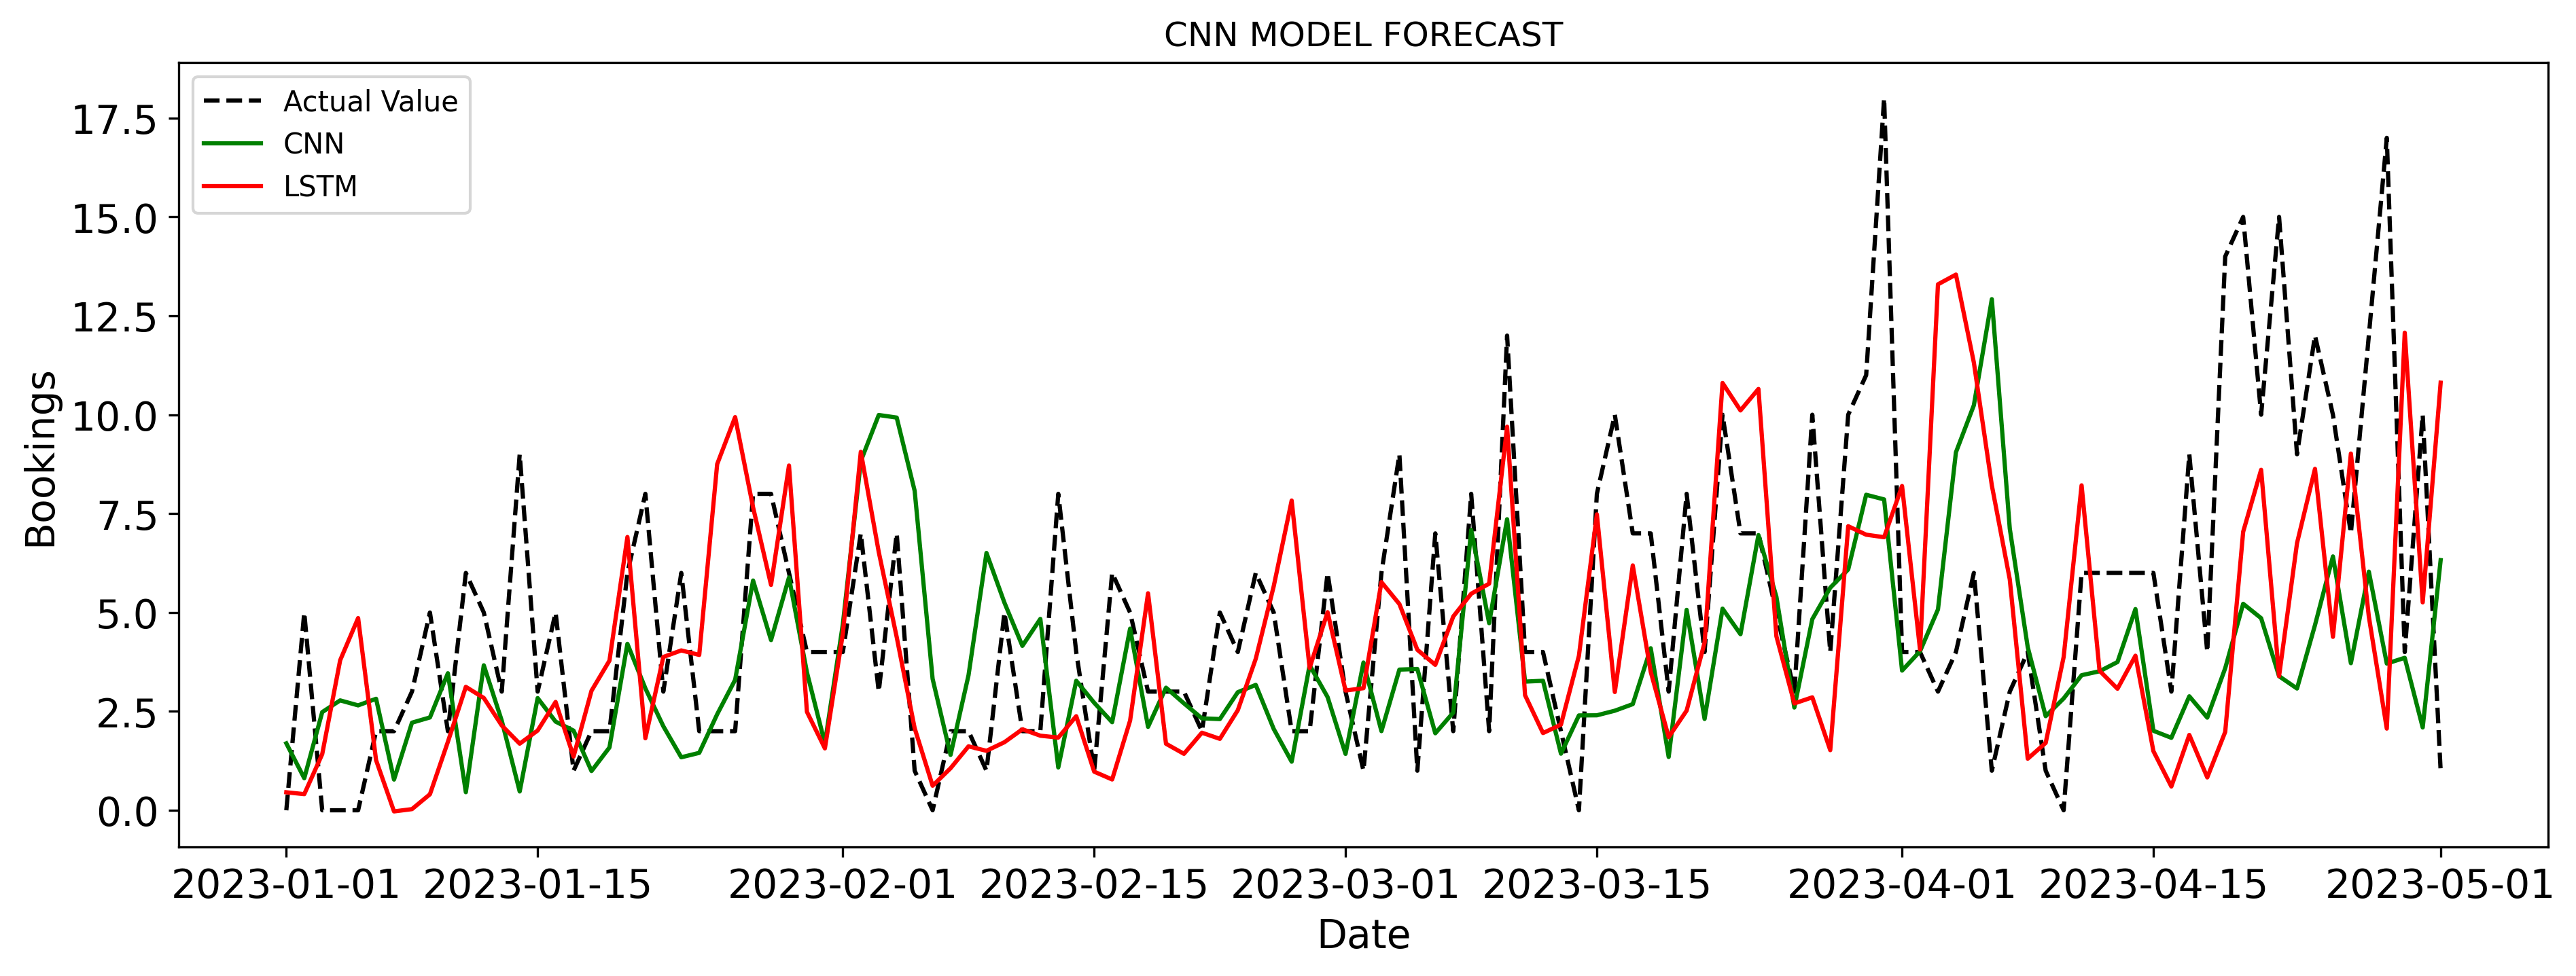
\includegraphics[width=14cm]{images/combined_prediction}
	\caption{Predictions of CNN 3 and LSTM 3 - [source:author]}
	\label{fig:combined_model}
\end{figure}

\subsection{Feature Engineering}
\label{sec:feature_eng}
Feature Engineering (FE) is used to create new input values also called features. Those values are further used to enhance a model's capability of learning. \cite{feature_eng_2} The approaches before used the whole timestamp \verb|tasTime_from| resulting that only one feature is available to train the models.  
Looking at the structure of a date like 2023-01-01 additional features become visible. Those values can be extracted and used to train the model.  The structure essentially hosts aspects like \verb|day of the month|, \verb|month|,\verb|year|, \verb|quarter of the year| as well as \verb|week of the year|. Furthermore this approach provides the possibility to provide additional context to the model like holidays. The insights gathered during chapter \ref{chap:insights} furthermore revealed  seasonal patterns. By extracting those characteristics form every single date more features become available to train the model. As the LSTM model in general looks like the more suitable candidate due to the past results it provided during section \ref{sec:implementation} and section \ref{sec:hyper} the approach of feature engineering is only applied onto the LSTM approach.
\newline
In order to extract additional features the following code is applied: 
\begin{lstlisting}
df['month'] = df.index.month
df['day'] = df.index.day
df['dayofweek'] = df.index.dayofweek
df['quarter'] = df.index.quarter
df['year'] = df.index.year
df["weekend"] = np.where(df.index.day_name().isin(['Saturday', 'Sunday']), 1, 0)
df['week_of_year'] = df.index.isocalendar().week
austrian_holidays = Austria(years=list(range(2017, 2024)))
df['holiday'] = df.index.map(lambda x: int(x in austrian_holidays))
df["main_season"] = np.where(df["month"].isin([5, 6, 7, 8, 9]), 1, 0)
df["off_season"] = np.where(df["month"].isin([5, 6, 7, 8, 9]), 0, 1)
df["ut"] = (df["bookings"] > high_ut).astype(float)
\end{lstlisting}
The initial dataframe remains untouched and got the same structure as in section \ref{sec:implementation}. As the index of the \verb|df| is initialised as \verb|pd.to_datetime()| operations like \verb|index.month|, \verb|index.day| etc. become available. Those functions extract the values based on each index available within the dataframe. 
For the initial training of the multivariate LSTM model the following architecture and parameters are used:
\begin{lstlisting}
Bidirectional(LSTM(120,return_sequences=True,
              input_shape=(X_train.shape[1],X_train.shape[2]))),
Bidirectional(LSTM(120,
              input_shape=(X_train.shape[1],X_train.shape[2]))),
Dropout(0.2),
Dense(1)

lstm_model.compile(
    loss=Huber(),
    optimizer=Adam(),
    metrics=['mae']
)

lstm_model.fit(
X_train, 
Y_train, 
epochs=200, 
)
\end{lstlisting}
As this model now utilises multiple features the parameter \verb|input_shape| needs to be set.  \verb|X_train.shape[1]| represents the number of timesteps whereas \verb|X_train.shape[2]| represents the number of features utilised for each timestep. Furthermore \verb|lstm_model.fit| receives now two input values whereas \verb|X_train| indicates the input features and \verb|Y_train| represents the actual output of a certain time step. For previous models only one input was required due to the way the data is structured. 
The training results of the model are highlighted in figure \ref{fig:lstm_multi_1_mae} and \ref{fig:lstm_multi_1_prediction} 
\begin{figure}[H]
	\centering
		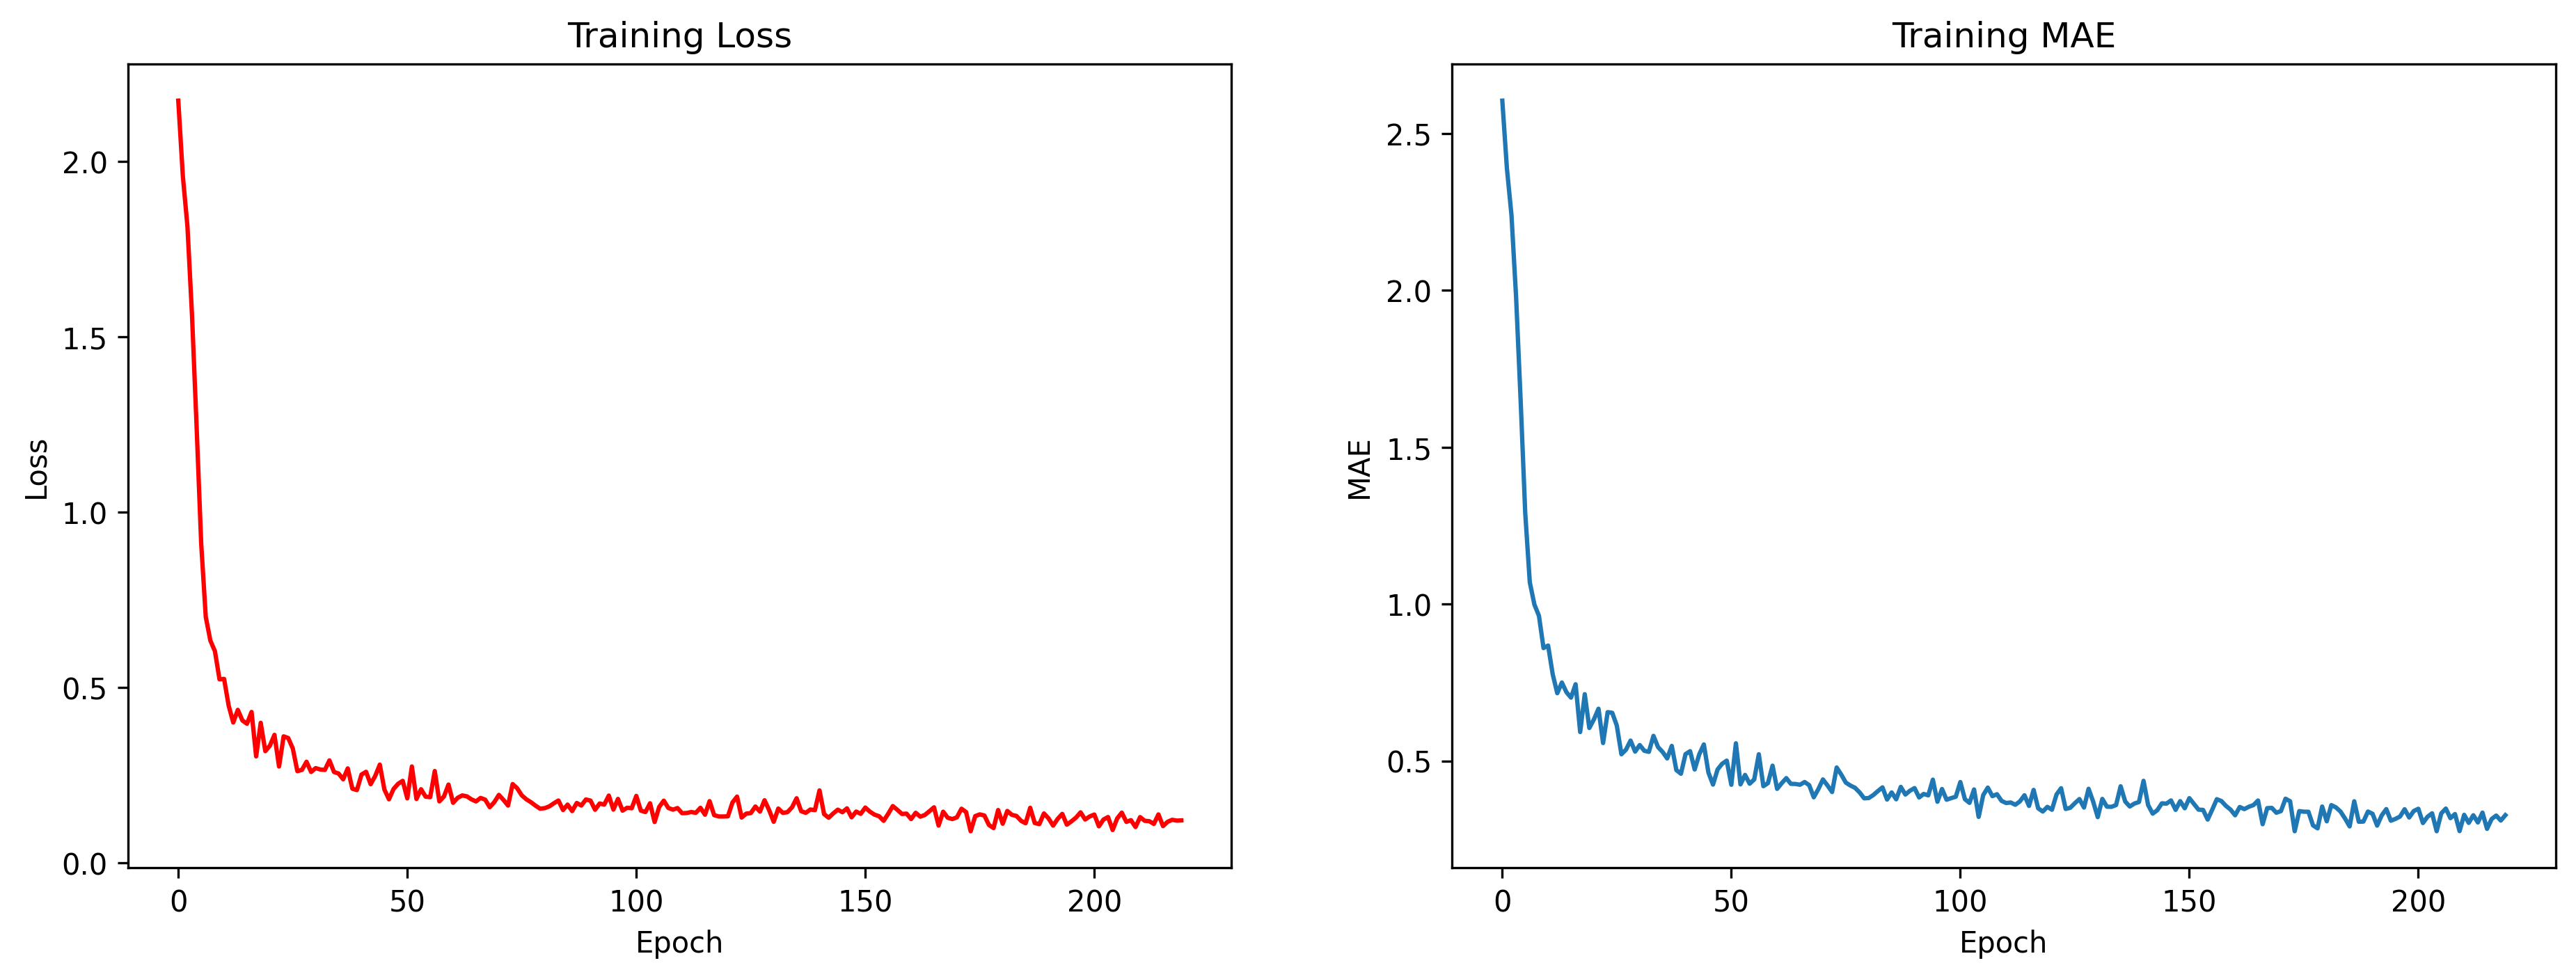
\includegraphics[width=12cm]{images/lstm_multi_1_mae}
	\caption{Change of Loss and MAE - [source:[author]]}
	\label{fig:lstm_multi_1_mae}
\end{figure}
Both the final loss (0.25) and MAE (0.30) are almost identical to the results achieved for the previous models. The major difference is the actual prediction results on the test data highlighted in figure \ref{fig:lstm_multi_1_prediction}. It is clear to see that the model's performance increased dramatically. This behaviour indicates that the model was overfitting the data and not being able to create accurate predictions on the test data. By increasing the context to the LSTM model utilising additional features the models performance on unseen data increased as well. 
\begin{figure}[H]
	\centering
		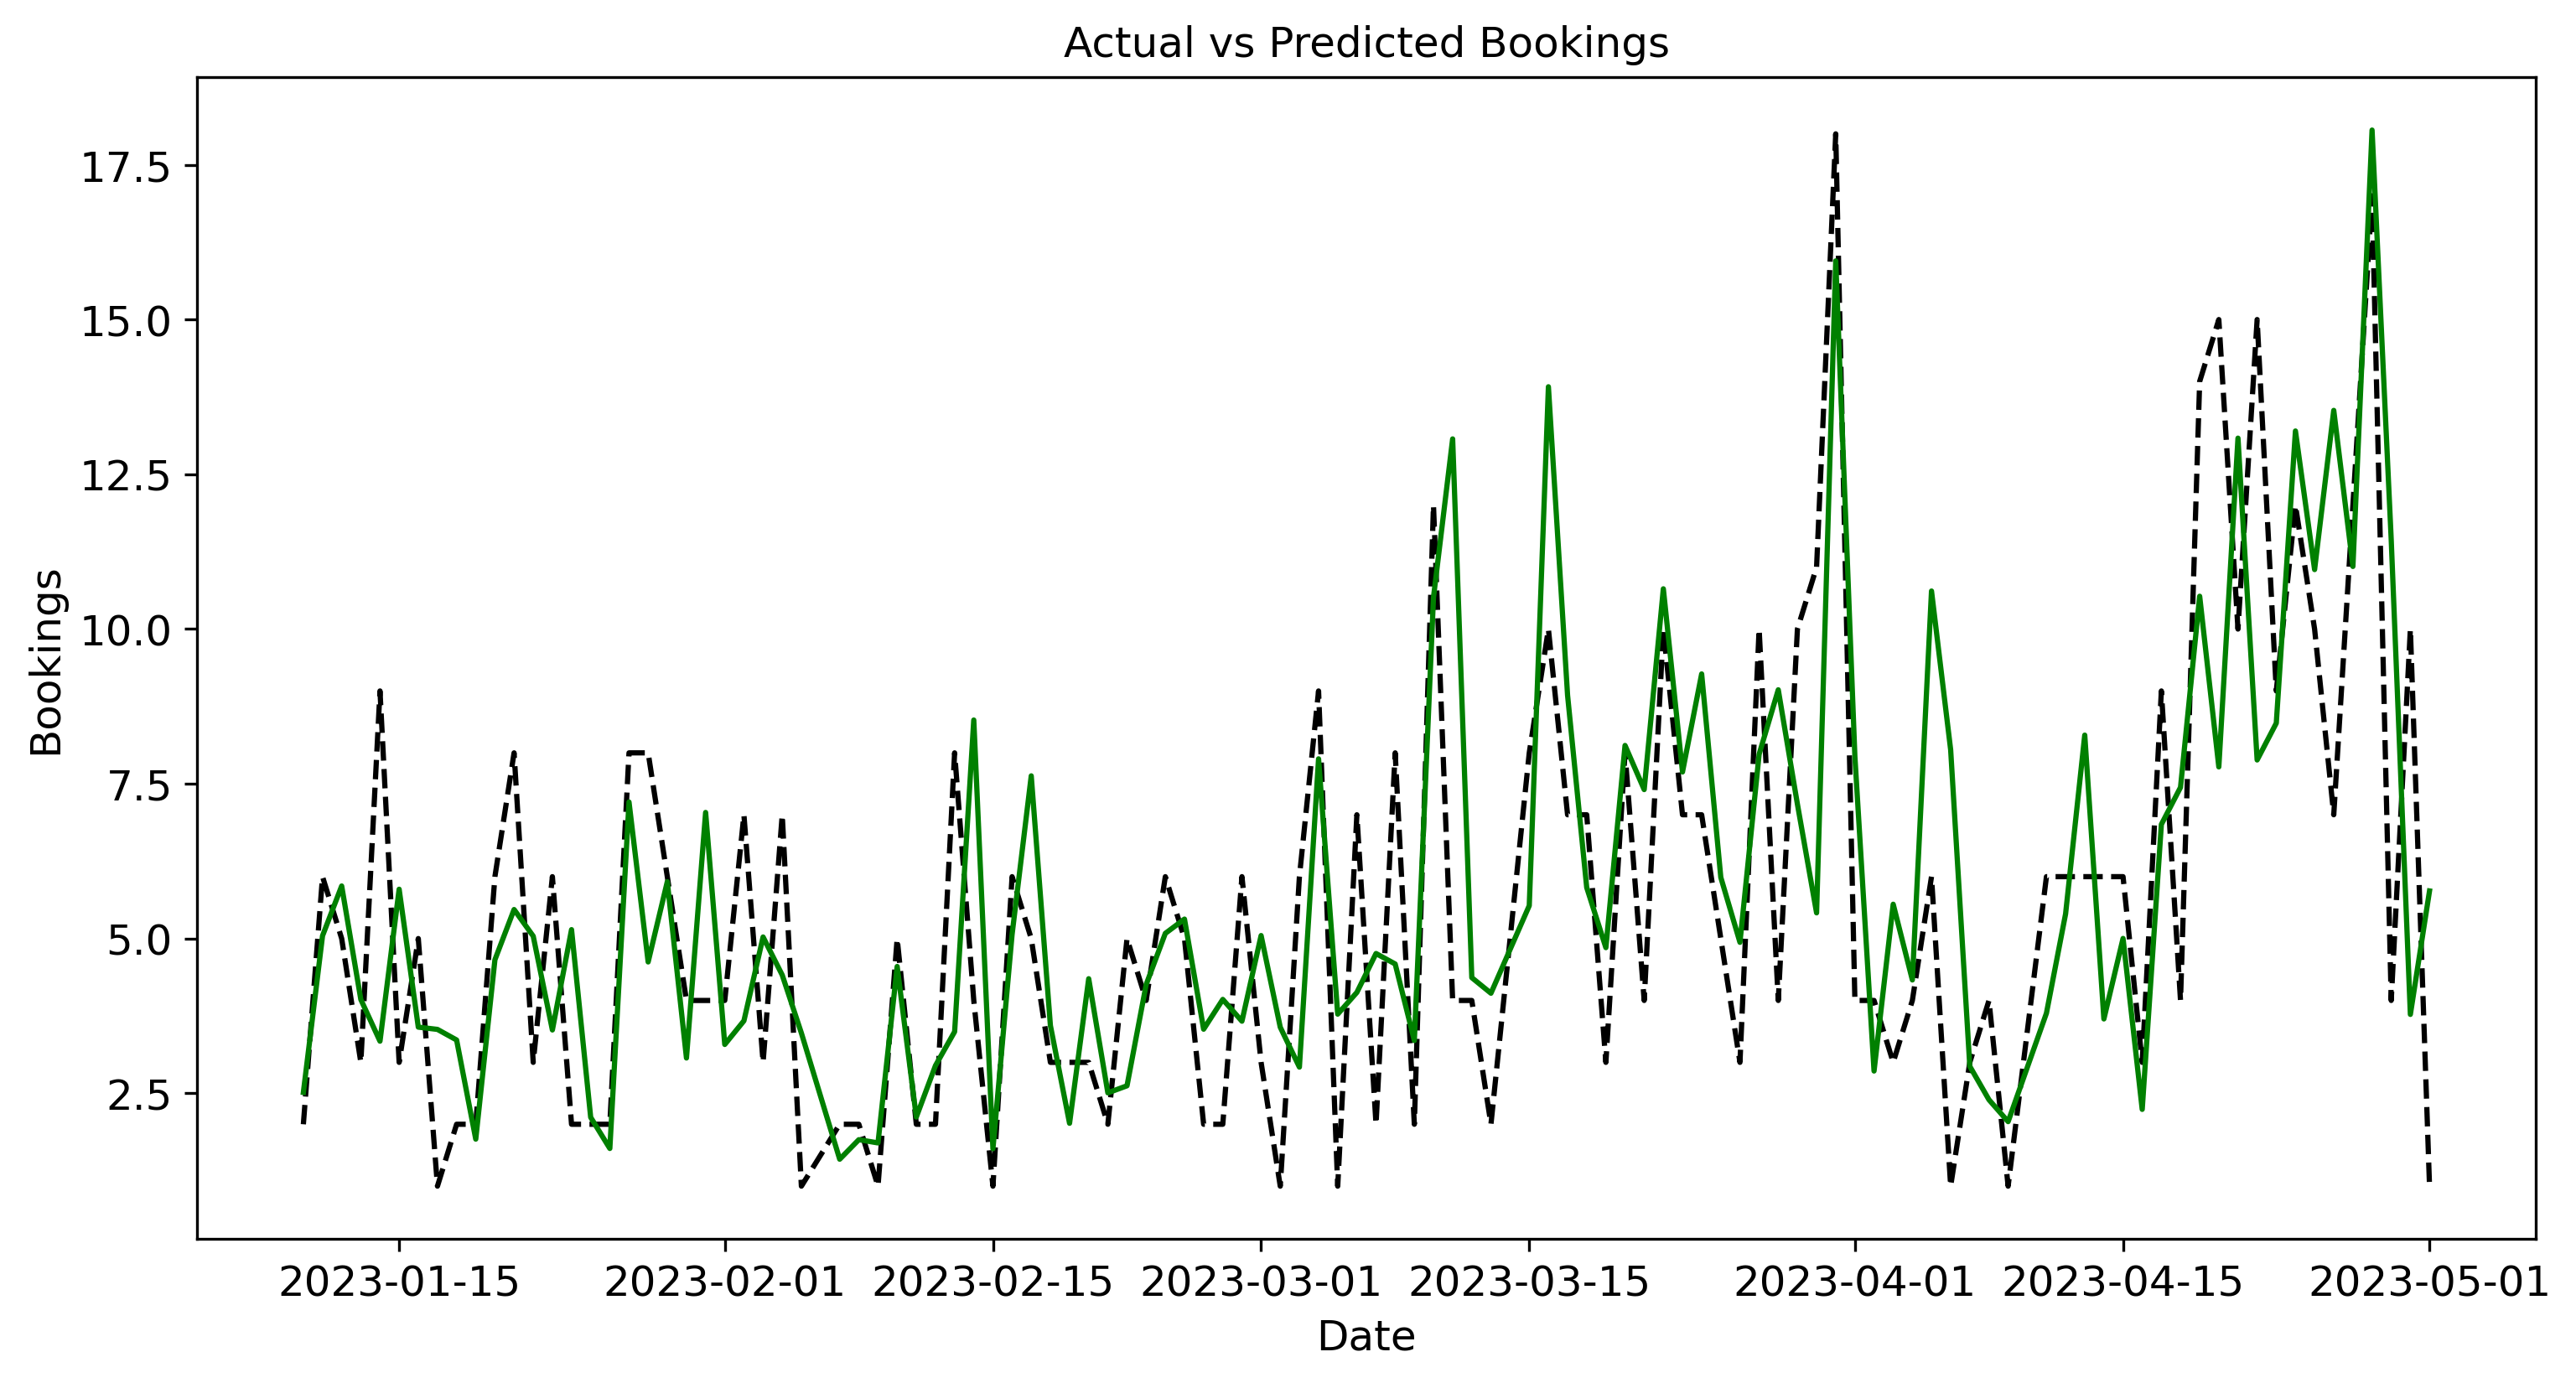
\includegraphics[width=14cm]{images/lstm_multi_1_prediction}
	\caption{Predictions on test set from 2023-01-01 to 01-05-2023 - [source:[author]]}
	\label{fig:lstm_multi_1_prediction}
\end{figure}
Looking at the results in figure \ref{fig:lstm_multi_1_prediction} the enhanced LSTM model is capable of catching up the trends present in the test data. Section \ref{sec:pred_and_ym} discusses the achieved results and whether or not the model can be used to support the current YM in place.

\section{Predictions and Yield Management}
\label{sec:pred_and_ym}
To determine whether or not the model can be utilised to support the YM knowledge about how far in advance buses are booked is crucial. By computing the median timespan utilising the attributes \verb|createdAt| and \verb|tasTime_from| this information can be gathered from the available dataset. The median timespan between \verb|createdAt| and \verb|taskFrom_time| is around 38 days. Throughout the whole implementation process which included the training of various model architectures as well as singelvariate and multivariate models, models utilizing LSTM achieved the best results. 

By looking at the final result achieved in figure \ref{fig:lstm_multi_1_prediction} it is clear to see that the model has the ability to predict future data. Although the results are not perfect for each day the model is able to recognise trends present in the test data. Whereas prediction might be off sometimes the achieved results still can be utilised to support the YM. As YM can have a tremendous influence on customers' decisions to whether or not they book a bus since it changes the pricing security mechanisms need to be set in place. On the one hand predictions are personally checked if they are feasible or not. Furthermore the predictions are set in context with previous years. This context involves seasonal trends and takes holidays in Austria, Germany, Switzerland and Liechtenstein into account. Especially predictions for Easter holidays are monitored since they might occur during different seasons. Additionally the model's performance is continuously monitored and a training schedule is set in place.
As the median for bookings in advance is around 38 days the results achieved for on the test data determine that this range can be predicted accurately.
%----------------------------------------------------------------
%
%  File    :  analytical_dashboard.tex
%
%  Authors : Thomas Lerchbaumer
% 
%  Created :  19 March 2022
% 
%  Changed :  19 March
% 
%----------------------------------------------------------------

\chapter{Implementation of Averages and Grouping}
\label{chap:analytical_dashboard}
Since this paper aims to extract metrics that can contribute to an analytical dashboard this section focuses on the implementation of various groupings as well as their visualisation. As the analytical dashboard is web based a short overview of its technical setup is given in section \ref{sec:tech_set}.

\section{Technical Setup}
\label{sec:tech_set}
As those implementations will contribute to an analytical dashboard the visualisation of the prepared data is implemented using React. For each grouping a separate React component is created. Communication between the front- and backend is accomplished using a Rest interface. 

\begin{itemize}
\item  \verb|React|\footnote{https://react.dev/} - used for visualization
\item \verb|Python|\footnote{https://www.python.org/} - used to implement the grouping logic and interaction with the database
\item \verb|fastapi|\footnote{https://fastapi.tiangolo.com/} - Rest interface (Connection between backend and frontend) 
\item \verb|geopy|\footnote{https://geopy.readthedocs.io/en/stable/} - used for calculations on latitude and longitude 
\end{itemize}
\section{Grouping Implementation}

\subsection{Grouping by Geographical Attributes}
The dataset for bus search requests (after cleaning) currently has around 230.000 entries. As the geographical calculations as well as the grouping logic are computational expensive tasks it is not feasible to redo this logic on every request. To enable real time requests with various filters onto the grouped data an additional database table is introduced. The table consists of two attributes: 
\begin{itemize}
\item \verb|parent_id (FK - search_requests(task_id)| - parent that defines a region 
\item \verb|child_id (FK - search_requests(task_id)| - entries that belong to a certain parent region  
\end{itemize}
This design comes along with several advantages. The logic for analytical requests and the grouping logic can be separated. Furthermore new entries for groupings can be added to a potential parent in a more efficient way as those entries only need to be compared to the attributes of \verb|parent_id|.

For geographical grouping the following logic is applied:
\begin{lstlisting}
radius = 20
    res = collections.defaultdict(list)
    tmp_list = collections.defaultdict(list)
    for point_a in data:
        tmp_point_a_dep = tuple((point_a['taskFrom_lng'], point_a['taskFrom_lat']))
        tmp_point_a_dest = tuple((point_a['taskTo_lng'], point_a['taskTo_lat']))
        key = point_a['id']
        found = False
        for key_b in res:
            point_b = res[key_b][0]

            tmp_point_b_dep = tuple((point_b['taskFrom_lng'], point_b['taskFrom_lat']))
            tmp_point_b_dest = tuple((point_b['taskTo_lng'], point_b['taskTo_lat']))
            actual_distance_dep = distance.great_circle(tmp_point_a_dep, tmp_point_b_dep).km
            actual_distance_dest = distance.great_circle(tmp_point_a_dest, tmp_point_b_dest).km
            if actual_distance_dep < radius and actual_distance_dest < radius:
                res[key_b].append(point_a)
                found = True
                break
        if not found:
            res[key].append(point_a)
\end{lstlisting}
This logic performs the comparison between two geographical entries. Whenever \verb|point\_b| is within a 20km radius of the departure and destination area from \verb|point\_a| \verb|point\_b| is added to the group from \verb|point\_a|. Utilizing the demonstrated database design makes it possible to still include filters like date ranges to filter groupings by date. Furthermore the averages for attributes explained in section \ref{sec:averages} can be utilized and compared to evaluate certain trends. By adjusting the logic above and removing the constraint that both destination and departure has to be within a certain range this data can further be grouped into popular destination places as well as popular departure places. Depending on the grouping technique various insights can be gathered. By analysing grouped data that mark routes (same departure/destination radius) the pricing strategy for routes with high demand can be adapted. Whereas analysing the grouping on departure places with high traffic bus operators might consider to expand their maximum approaching distance. Furthermore by changing the way how the data is fetched from the database by querying results where no bus was offered \verb|amountSearchResults == 0| a different grouping becomes available for analysing. 
\subsubsection{Visualisation}
Depending on how the entries are grouped different visualization techniques are applied. To detect departure areas with high demand a heatmap is utilised. Therefore an interactive map is utilized. Onto this map areas with high demands are plotted following a color scheme. Red circles indicate high demand whereas blue areas indicate areas with less demand as shown in figure \ref{fig:heatmap_dep}. Furthermore this visualization can be filtered by applying date ranges. Additionally areas with high demand are displayed in a table including total count of requests for a certain area, average pax as well as the average travel distance.
\newline
As a heatmap is not suitable to visualise the grouped routes those groupings are displayed using a table. Additionally the table is filterable by date in order to be able to analyse the data split up into certain time periods. Furthermore the table hosts information about average pax and average travel distance. 
\begin{figure}[H]
	\centering
		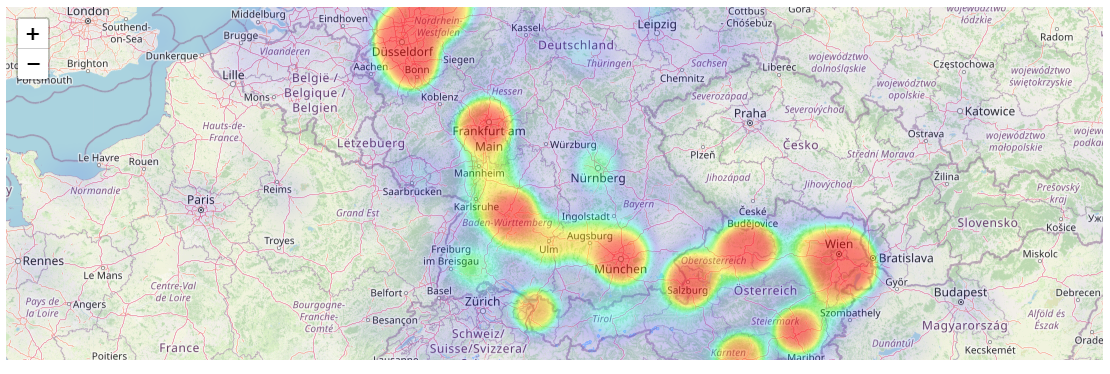
\includegraphics[width=15cm]{images/heatmap_dep}
	\caption{Interactive heatmap highlighting departure places with high demand - [source:[author]]}
	\label{fig:heatmap_dep}
\end{figure}


\subsection{Grouping by Time}
In contrast to geographical grouping, groupings by time do not require a table within the database in order to process requests in real time. To group requests by time the following logic is applied to the fetched data: 
\begin{lstlisting}
def group_requests_by_time(data):
    df = pd.DataFrame(data)
    df = pd.to_datetime(df[0])
    grouped = df.groupby(df.dt.hour).count()
    for name in grouped.index:
        tmp = {"x": str(name) + ":00", "y": int(grouped.loc[name])}
        res[0]['data'].append(tmp)
    return res
\end{lstlisting}
To group search requests by days the following logic is applied: 
\begin{lstlisting}
def group_requests_by_day(data):
    data_format = pd.DataFrame(data)
    data_format = pd.to_datetime(data_format[0], format='%Y-%m-%d %H:%M:%S')
    grouped = data_format.groupby([data_format.dt.year, data_format.dt.month, data_format.dt.day]).count()
    res = []
    for name in grouped.index:
        date = str(name[0]) + "-" + str(name[1]) + "-" + str(name[2])
        tmp = {"value": int(grouped.loc[name]), "day": date}
        res.append(tmp)
    res = sorted(res, key=lambda x: x['day'])
    return res
\end{lstlisting}
Depending on which attribute e.g. \verb|createdAt| or \verb|taskFrom_time| is fetched from the database different groupings become available. Both attributes provide valuable information. When the data is grouped by utilising the attribute \verb|createdAt| the success rate of previous marketing campaigns can be evaluated. Furthermore this information can be consulted to plan future marketing campaigns. By grouping the data using the attribute \verb|taskFrom_time| seasonal patterns become visible as shown in \ref{fig:dep_grouping}
\subsubsection{Visualisation}
The hourly groupings are visualised using a line chart as demonstrated in figure \ref{fig:hourly_grouping}.
\begin{figure}[H]
	\centering
		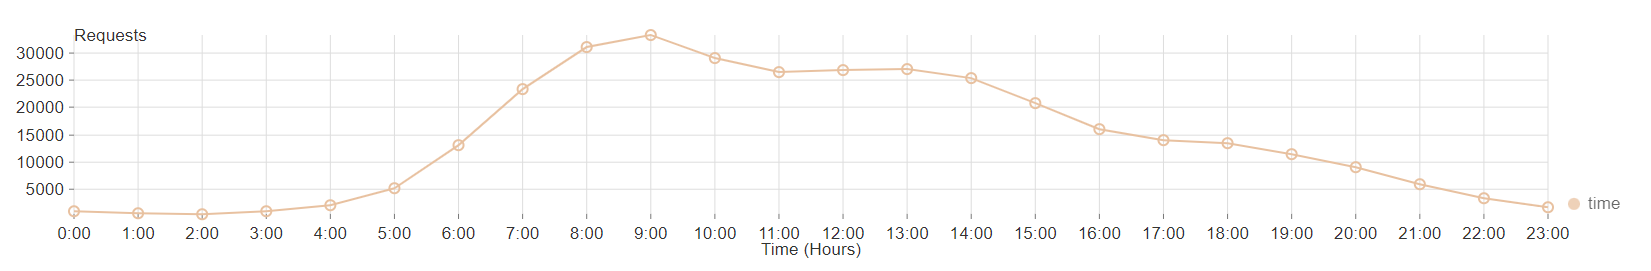
\includegraphics[width=15cm]{images/requests_hour}
	\caption{***PLACEHOLDER Requests grouped on hourly basis- [source:[author]]}
	\label{fig:hourly_grouping}
\end{figure}
By analysing figure \ref{fig:hourly_grouping} the highest number of the most search requests are made at around 9 am. By hovering over each data point the amount of search requests become visible. 
\newline
 
\begin{figure}[H]
	\centering
		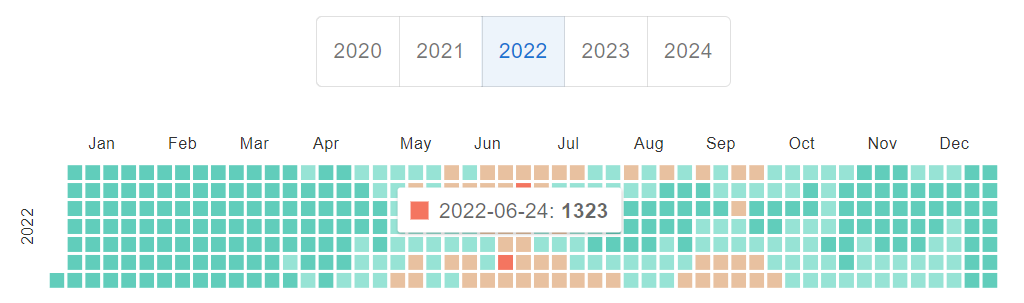
\includegraphics[width=15cm]{images/grouping_by_taskFrom}
	\caption{ **PLACEHOLDER Daily grouping of departure dates- [source:[author]]}
	\label{fig:grouping_dep_daily}
\end{figure}
The grouping by day is visualized by a heatmap mapped to an calendar. By investigating the results for different years seasonal patterns become visible.
\begin{figure}[H]
	\centering
		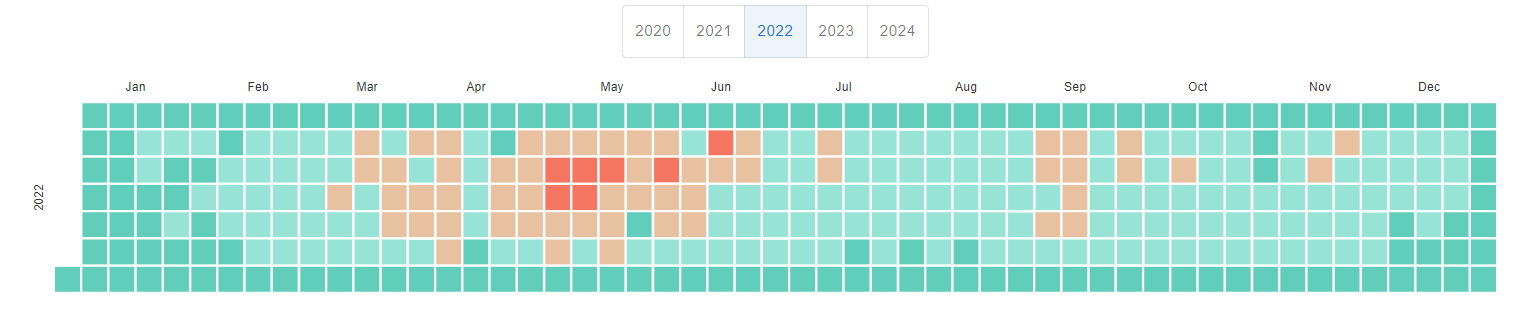
\includegraphics[width=15cm]{images/grouping_by_created_at}
	\caption{**PLACEHOLDER Daily grouping of when search requests are made- [source:[author]]}
	\label{fig:grouping_search_daily}
\end{figure}
All of the extracted groupings are filterable by date ranges in real time. Furthermore whenever a filter is applied the average pax as well as the average distance is provided to the user.
% --- Bibliography ------------------------------------------------------

%IEEE Citation [1]
\bibliographystyle{IEEEtran}
%for alphanumeric citation eg.: [ABC19]
%\bibliographystyle{alpha}

% List references I definitely want in the bibliography,
% regardless of whether or not I cite them in the thesis.

\newpage
\addcontentsline{toc}{chapter}{Bibliography}
\bibliography{testBib}

\newpage

% --- List of Figures ----------------------------------------------------

\addcontentsline{toc}{chapter}{List of Figures}
\listoffigures


% --- List of Tables -----------------------------------------------------

\newpage
\addcontentsline{toc}{chapter}{List of Tables}
\listoftables

% --- Appendix A -----------------------------------------------------

\backmatter
\appendix
\begin{appendices}
\chapter{Appendix}

(Hier können Schaltpläne, Programme usw. eingefügt werden.)

\clearpage
\end{appendices}

\end{document}
